\documentclass[
version=last,toc=bib,toc=graduated,toc=index,toc=listof,fontsize=9pt,openany]{scrbook}
%\pdfminorversion=4
\usepackage{polyglossia}
\setdefaultlanguage{english}

\setmainfont{Source Sans Pro}
\setsansfont{Source Sans Pro}

\usepackage{ifmtarg}
\usepackage{ifthen}
\usepackage{etoolbox} % \ifstrempty

\usepackage{geometry}
\geometry{%a6paper
paperwidth=125mm, paperheight=168mm, 
portrait,
top=22mm,
inner=22mm,
outer=20mm,
bottom=25mm,
headsep=3mm,
footskip=12mm
}

% math symbols
\usepackage{amssymb}

\usepackage{ragged2e} % nicer typesetting (hyphenation) for non raggedright and raggedleft
\usepackage{lscape}
\setlength{\parskip}{0pt}

\usepackage{relsize}

\clubpenalty=10000
\widowpenalty=10000 
\displaywidowpenalty=10000

\usepackage[]{microtype}

\usepackage{graphicx} % graphics

% search path for images
\graphicspath{{images-print/}{icons/}{extra-pages/}{wallpaper/}}
\usepackage{wrapfig}  % sponsor logos wrapped with text

\usepackage{tabu}
\usepackage[table,cymk]{xcolor}
\usepackage{colortbl}

% embed PDF pages
% pdfpages must not be loaded before colortbl!
\usepackage{pdfpages}
% TikZ must not be loaded before colortbl
\usepackage{tikz}
\usetikzlibrary{calc}

\usepackage{multirow}
%\usepackage{booktabs}

\usepackage{array}

% multiple text columns (list of thanks)
\usepackage{multicol}

\usepackage{refcount} % calculation of the page where the map is located

\usepackage{qrcode} % QR codes with plain TeX/LaTeX

\usepackage{mathabx} % diamond symbol in the menu

% page background
\usepackage[manualmark]{scrlayer-scrpage}
\pagestyle{scrplain}

\newcommand{\acro}[1]{{\textsmaller{#1}}} % macro for abbreviations with more than one capitalised letter


% title/metadata
\title{State of the Map 2019}
\subtitle{Programme}
\author{OpenStreetMap Foundation}
\date{\today}

\clearscrheadings

% page numbers
\cfoot[\begin{small}\pagemark\end{small}]{\begin{small}\pagemark\end{small}}
\ofoot[]{}
\ifoot[]{}
\pagestyle{scrplain}

\linespread{1.15}

% include our custom macros
% command for a new time slot
\newcommand{\talkTime}{9:99}
\newcommand{\newTimeslot}[1]{\newpage\renewcommand{\talkTime}{#1}}

% new time slot but without a pagebreak
\newcommand{\newSmallTimeslot}[1]{\renewcommand{\talkTime}{#1}}

% initialise \conferenceDay
\newcommand{\conferenceDay}{Noday}


% define default page style (cutting marks with page number)
\DeclareNewLayer[background, oddorevenpage, width=125mm,%
height=169mm, contents={%
  
\includegraphics{wallpaper/crop-marks.pdf}%
}]{cropmarksevery}
\newpairofpagestyles[scrheadings]{cropmarksstyle}{}
\AddLayersAtBeginOfPageStyle{cropmarksstyle}{cropmarksevery}

% page style for title pages
\DeclareNewLayer[background, oddorevenpage, width=125mm,%
height=169mm, contents={%
  
\includegraphics{wallpaper/front-cover-with-crop-marks.pdf}%
}]{titlelayer}
\newpairofpagestyles[]{titlestyle}{}
\AddLayersAtBeginOfPageStyle{titlestyle}{titlelayer}

% define alias commands for all three days
\def\saturday{Saturday}
\def\sunday{Sunday}
\def\monday{Monday}

% define Saturday page style
\DeclareNewLayer[background, oddpage,  width=125mm,%
height=169mm, contents={%
  
\includegraphics{wallpaper/saturday-odd.pdf}%
}]{saturdayodd}
\DeclareNewLayer[background, evenpage,  width=125mm,%
height=169mm, contents={%
  
\includegraphics{wallpaper/saturday-even.pdf}%
}]{saturdayeven}
\DeclareNewLayer[background, oddpage,  width=125mm,%
height=169mm, contents={%
  
\includegraphics{wallpaper/saturday-odd-rotated.pdf}%
}]{saturdayoddrotated}
\newpairofpagestyles[scrheadings]{saturday-table}{}
\AddLayersAtBeginOfPageStyle{saturday-table}{saturdayeven}
\AddLayersAtBeginOfPageStyle{saturday-table}{saturdayoddrotated}
\newpairofpagestyles[scrheadings]{saturday}{}
\AddLayersAtBeginOfPageStyle{saturday}{saturdayeven}
\AddLayersAtBeginOfPageStyle{saturday}{saturdayodd}

% define Sunday page style
\DeclareNewLayer[background, oddpage,  width=125mm,%
height=169mm, contents={%
  
\includegraphics{wallpaper/sunday-odd.pdf}%
}]{sundayodd}
\DeclareNewLayer[background, evenpage,  width=125mm,%
height=169mm, contents={%
  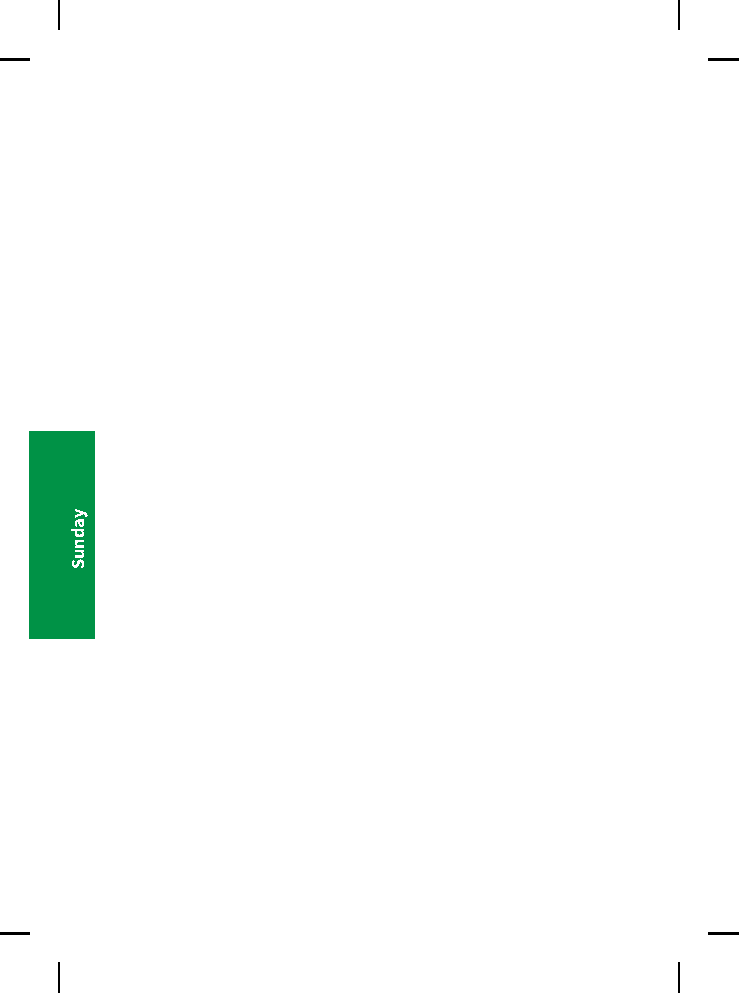
\includegraphics{wallpaper/sunday-even.pdf}%
}]{sundayeven}
\DeclareNewLayer[background, oddpage,  width=125mm,%
height=169mm, contents={%
  
\includegraphics{wallpaper/sunday-odd-rotated.pdf}%
}]{sundayoddrotated}
\newpairofpagestyles[scrheadings]{sunday-table}{}
\AddLayersAtBeginOfPageStyle{sunday-table}{sundayeven}
\AddLayersAtBeginOfPageStyle{sunday-table}{sundayoddrotated}
\newpairofpagestyles[scrheadings]{sunday}{}
\AddLayersAtBeginOfPageStyle{sunday}{sundayeven}
\AddLayersAtBeginOfPageStyle{sunday}{sundayodd}

% define Monday page style
\DeclareNewLayer[background, oddpage,  width=125mm,%
height=169mm, contents={%
  
\includegraphics{wallpaper/monday-odd.pdf}%
}]{mondayodd}
\DeclareNewLayer[background, evenpage,  width=125mm,%
height=169mm, contents={%
  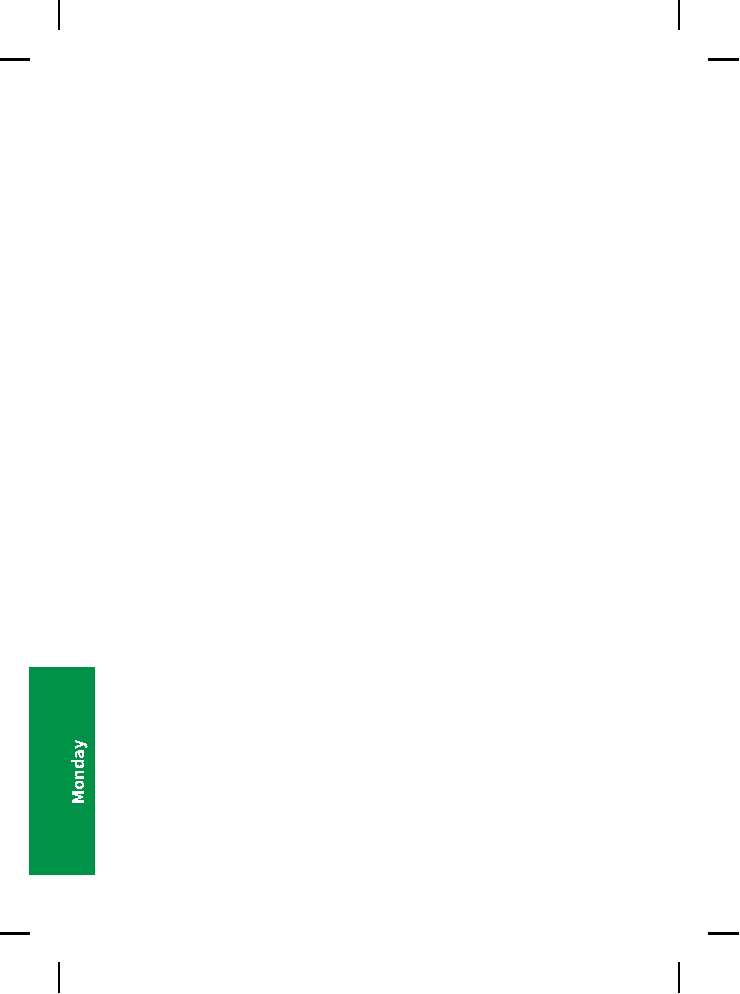
\includegraphics{wallpaper/monday-even.pdf}%
}]{mondayeven}
\DeclareNewLayer[background, oddpage,  width=125mm,%
height=169mm, contents={%
  
\includegraphics{wallpaper/monday-odd-rotated.pdf}%
}]{mondayoddrotated}
\newpairofpagestyles[scrheadings]{monday-table}{}
\AddLayersAtBeginOfPageStyle{monday-table}{mondayeven}
\AddLayersAtBeginOfPageStyle{monday-table}{mondayoddrotated}
\newpairofpagestyles[scrheadings]{monday}{}
\AddLayersAtBeginOfPageStyle{monday}{mondayeven}
\AddLayersAtBeginOfPageStyle{monday}{mondayodd}

% \setpagebackground selects the page style to be used depending on the current day. Each day has
% its own page style.
\newcommand{\setPageBackground}{ %
  \ifthenelse{\equal{\conferenceDay}{\saturday}}{%
    \pagestyle{saturday}
  }{}
  \ifthenelse{\equal{\conferenceDay}{\sunday}}{%
    \pagestyle{sunday}
  }{}
  \ifthenelse{\equal{\conferenceDay}{\monday}}{%
    \pagestyle{monday}
  }{}
}


% additional column type for tables
\newcolumntype{Y}[1]{>{\RaggedRight\arraybackslash}p{#1}}

%% length of the title boxes
\newlength{\titleboxwidth}
\advance\titleboxwidth by -6pt

\newlength{\roomWidth}
\newlength{\timeWidth}
\newlength{\roomTimeWidth}
\newlength{\titleWidth}
\newcommand{\tmpRoomTimeWidth}{}
\newcommand{\tmpTitleWidth}{}

\newcommand{\setAbstract}[6]{%
  % 1. speaker
  % 2. title
  % 3. subtitle
  % 4. abstract (Text)
  % 5. colour
  % 6. room
  \setPageBackground%
  \calculateRoomTimeAndTitleWidth{#1}{#6}%
  \noindent\fcolorbox{white}{#5}{%
    \parbox{\titleboxwidth}{%
      \isSpeakerEmpty{#1}{#2}{#6}%
      \isSubtitleEmpty{#3}%
    }%
  }%
  %
  \isAbstractEmpty{#4}%
  \vspace{0.5em}% space to the next talk even if there is no abstract
}

% Calculate width of title and room/time field
% Arguments: speaker, room
\makeatletter
  \newcommand{\calculateRoomTimeAndTitleWidth}[2]{%
    \@ifmtarg{#1}{% speaker is empty
      \settowidth{\roomWidth}{#2, \talkTime}%
    }{% speaker is not empty
      \settowidth{\roomWidth}{#2}%
    }%
    \settowidth{\timeWidth}{\talkTime}%
    \directlua{require("lua/titleWidth")}%
    \setlength{\titleboxwidth}{\directlua{getTitleBoxWidth()}}%
    \renewcommand{\tmpRoomTimeWidth}{\directlua{getTimeRoomWidth()}}%
    \setlength{\roomTimeWidth}{\tmpRoomTimeWidth}%
    \renewcommand{\tmpTitleWidth}{\directlua{getTitleWidth()}}%
    \setlength{\titleWidth}{\tmpTitleWidth}%
  }%
\makeatother

% Lay out the subtitle
% has to be a separate function and has to be surrounded by \makeatletter for technical reasons
\makeatletter
  \newcommand{\isSubtitleEmpty}[1]{%
    \@ifnotmtarg{#1}{%
      \par
      \RaggedRight
      \vspace{0.5\baselineskip}
      \noindent%
      \bfseries%
      #1%
    }
  }
\makeatother

% lay out the speaker if there is any
% We assume that there is only a subtitle if the talk has a speaker.
\makeatletter
  \newcommand{\isSpeakerEmpty}[3]{%
    % Arguments:
    % 1. speaker
    % 2. title
    % 3. room
    \@ifmtarg{#1}{%
      \begin{minipage}[t][][t]{\titleWidth}
        \RaggedRight
        \noindent%
        {\large \sectfont #2}%
      \end{minipage}%
      \hfill
      \begin{minipage}[t][][t]{\roomTimeWidth}
        \RaggedLeft%
        \noindent #3, \talkTime%
      \end{minipage}%
    }%
    {%
      \begin{minipage}[t][][t]{\titleWidth}
        \RaggedRight
        \emph{#1} % speaker
        \par%
        \vspace{0.3\baselineskip}
        \noindent%
        {\large \sectfont #2}%
      \end{minipage}%
      \hfill
      \begin{minipage}[t][][t]{\roomTimeWidth}
        \RaggedLeft
        \talkTime%
        \par%
        \noindent #3% room
      \end{minipage}%
    }%
  }
\makeatother

% Lay out the abstract if there is any
% has to be a separate function and has to be surrounded by \makeatletter for technical reasons
\makeatletter
\newcommand{\isAbstractEmpty}[1]{%
  \ifstrempty{#1}{%
    \vspace{1.5em}%
  }{%
    \vspace{0.5em}\newline%
    #1 \par% % abstract
    \vspace{1.5em}% space to the next talk even if there is an abstract
  }%
}
\makeatother

% define colours
\definecolor{GHS}{cmyk}{0.16 0 .05 0}
\definecolor{HSO}{cmyk}{0.02 0 0.12 0.11}
%\definecolor{academic}{cmyk}{0 0.02 0.23 0}
\definecolor{academic}{cmyk}{0.35 0 0.33 0.16}
\definecolor{HSW}{cmyk}{0.35 0 0.33 0.16}
\definecolor{KHS}{cmyk}{0 .24 0.29 .04}
\definecolor{Mathematikon C}{cmyk}{.16 0 0.35 0}
\definecolor{ochsenblutrot}{cmyk}{0 0.72 0.65 0.65}

% session at GHS
\newcommand{\abstractGHS}[4]%
{%
  \setAbstract{#1}{#2}{#3}{#4}{GHS}{GHS}
}

% abstract at HSO
\newcommand{\abstractHSO}[4]%
{%
  \setAbstract{#1}{#2}{#3}{#4}{HSO}{HSO}
}

% abstract for academic talks
\newcommand{\abstractAcademic}[4]%
{%
  \setAbstract{#1}{#2}{#3}{#4}{academic}{HSW}
}

% abstract at HSW
\newcommand{\abstractHSW}[4]%
{%
  \setAbstract{#1}{#2}{#3}{#4}{HSW}{HSW}
}

% abstract at KHS
\newcommand{\abstractKHS}[4]%
{%
  \setAbstract{#1}{#2}{#3}{#4}{KHS}{KHS}
}

% abstract at Mathematikon C
\newcommand{\abstractMathematikonC}[4]%
{%
  \setAbstract{#1}{#2}{#3}{#4}{Mathematikon C}{Mathematikon C}
}

% abstract at a different location
\newcommand{\abstractOther}[5]%
{%
  \setAbstract{#1}{#2}{#3}{#4}{commongray}{#5}
}

% infobox for workshops (they don't have an abstract in the booklet)
\newcommand{\workshopbox}[3]{%
  % 1. titel
  % 2. speaker
  % 3. Room
  \setlength\tabcolsep{0pt}
  \noindent\fcolorbox{white}{dezentrot}{%
    \parbox{\titleboxwidth}{%
      \noindent%
      \begin{tabu}{X[5L]r}
        \emph{#2} % Sprecher
        &
        \talkTime
        \tabularnewline
        {\noindent\large \bfseries #1}% % title
        &
        #3
        \tabularnewline
      \end{tabu}
    }
  }
  \setlength\tabcolsep{6pt} % set column padding back to default
}

% too long
\newcommand{\tooLong}{Dieser Text ist viel zu lang. Dieser Text ist viel zu lang. Dieser Text ist viel zu lang. Dieser Text ist viel zu lang. Dieser Text ist viel zu lang. Dieser Text ist viel zu lang. Dieser Text ist viel zu lang. Dieser Text ist viel zu lang. Dieser Text ist viel zu lang. Dieser Text ist viel zu lang. Dieser Text ist viel zu lang. Dieser Text ist viel zu lang. Dieser Text ist viel zu lang. Dieser Text ist viel zu lang. }

\newlength{\fboxwidth}

\def\workshopsSection{workshopsSection}
\def\abstractsSection{abstractsSection}

% boxes for text-only advertisement texts by our sponsors
\newcommand{\sponsorBox}[4]{%
  \setlength{\fboxwidth}{\textwidth}
  \advance\fboxwidth by -7.0pt
  \abstractSponsorbox{#1}{#2}{#3}{#4}{\workshopsSection}%
}

\newcommand{\sponsorBoxA}[4]{%
  \setlength{\fboxwidth}{\textwidth}
  \advance\fboxwidth by -10.0pt
  \abstractSponsorbox{#1}{#2}{#3}{#4}{\abstractsSection}%
}

%% store \parindent in separate variable because it is resetted to 0 in parboxes
\newlength{\saveparindent}
\setlength{\saveparindent}{\parindent}

%% box for advertisment by a sponsor
%% 1. logo
%% 2. width of the logo
%% 3. number of required lines of the logo (due to usage of wrapfigure)
%% 4. text
%% 5. Umfeld (\workshopsSection oder \abstractsSection}
\makeatletter
  \newcommand{\abstractSponsorbox}[5]{%
    \setlength{\fboxsep}{4.5pt}%
    \noindent%
    \ifthenelse{\equal{#5}{\workshopsSection}}{%
      \hspace{2.65pt}%
    }{%
      \hspace{-1pt}%
    }%
    \fcolorbox{gray}{white}{%
      \parbox{\fboxwidth}{
        \setlength{\parindent}{\saveparindent}%
        \@ifmtarg{#1}{}{%
          \begin{wrapfigure}[#3]{r}[0pt]{#2}
            \centering\vspace{-1\baselineskip}
            \includegraphics[width=#2]{#1}
          \end{wrapfigure}
        }

        \noindent #4
      }%
    }
    \setlength{\fboxsep}{3pt}
  }
  \setlength{\fboxsep}{3pt}
\makeatother

% definition of column types for the schedule tables
\newcolumntype{Z}[1]{>{\RaggedRight\arraybackslash}p{#1}}%
\newcolumntype{C}[1]{>{\Centering\arraybackslash}p{#1}}%

% common implementation of typesetting of a session in the tables
\newcommand{\talkInternal}[2]{%
  \textbf{#1}
  \ifthenelse{\equal{#2}{}}{}{%
    \newline\emph{#2}%
  }
}

% macro to typeset a talk in the schedule tables spanning over more than one row:
% usage: \longTalk{rowcount}{title}{speaker}
\newcommand{\longTalk}[3]{%
  &
  \multirow{#1}{\linewidth}{%
    \parbox{\linewidth}{
      %HACK Inserting a \vspace here is a dirty hack but it works.
      \vspace{0.45\baselineskip}
      \talkInternal{#2}{#3}%
    }
  }%
}%

% macro to typeset a talk in the schedule tables:
% usage: \talk{title}{speaker}
\newcommand{\talk}[2]{%
  &
  \talkInternal{#1}{#2}%
}%


% macro to typeset a talk in the schedule tables spanning over more than one column:
% usage: \multiColTalk{columns}{columnSpecs}{title}{speaker}
\newcommand{\multiColTalk}[4]{%
  &
  \multicolumn{#1}{#2}{\talkInternal{#3}{#4}}%
}%

\newcommand{\workshop}[3]%
{%
  \workshopbox{#1}{#2}{#3}
}%

\newcommand{\otherevent}[1]%
{%
  & \textbf{#1}
}%

\newcommand{\audimaxEvent}[2]%
{%
  &
  \multicolumn{3}{c}{
    \textbf{#1} (Audimax) \par \emph{#2}
  }
}%

\newcommand{\coffeespace}{\vspace{0.4em}}
\newcommand{\workshopspace}{\vspace{0.5em}\\}

% define colors
\definecolor{commongray}{gray}{.9}
\definecolor{tableRuleGray}{gray}{.4}
\definecolor{textGray}{gray}{.45}

% macro for table rules
\newcommand{\programCRule}[1]{%
  \arrayrulecolor{tableRuleGray}%
  \cdashline{#1}[0.2mm/0.4mm]%
}
\newcommand{\programHRule}[1]{%
  \arrayrulecolor{tableRuleGray}%
  \cdashline{2-#1}[0.2mm/0.4mm]%
}

% macro for empty session slots
\newcommand{\bookableSpace}{
  &
  \emph{\textcolor{textGray}{bookable space}}%
}

% diamond symbol for shortened titles
\newcommand{\diamondSymbol}{%
  \textsuperscript{%
    \diamond%
  }%
}

% speaker affiliation
\newcommand{\speakerAffiliation}[1]{%
  (#1)%
}

% lightning talk (title and author)
\newcommand{\lightningTalk}[2]{%
  \item \emph{#2:} #1%
}

% macro for no-video icon
\newcommand{\noVideo}{%
  
\includegraphics[height=9pt]{novideo.pdf}%
}

% skip line to make right/left table columns align
\newcommand{\skipline}{%
  \vspace{0.365cm}
}

% Ministerium für Verkehr advertisement (left)
%TODO get rid of their cropmarks, add ours
\DeclareNewLayer[background,%
  width=115mm,%
  height=158mm,%
  hoffset=5mm,%
  voffset=5mm,%
  contents={%
    %TODO correct size
    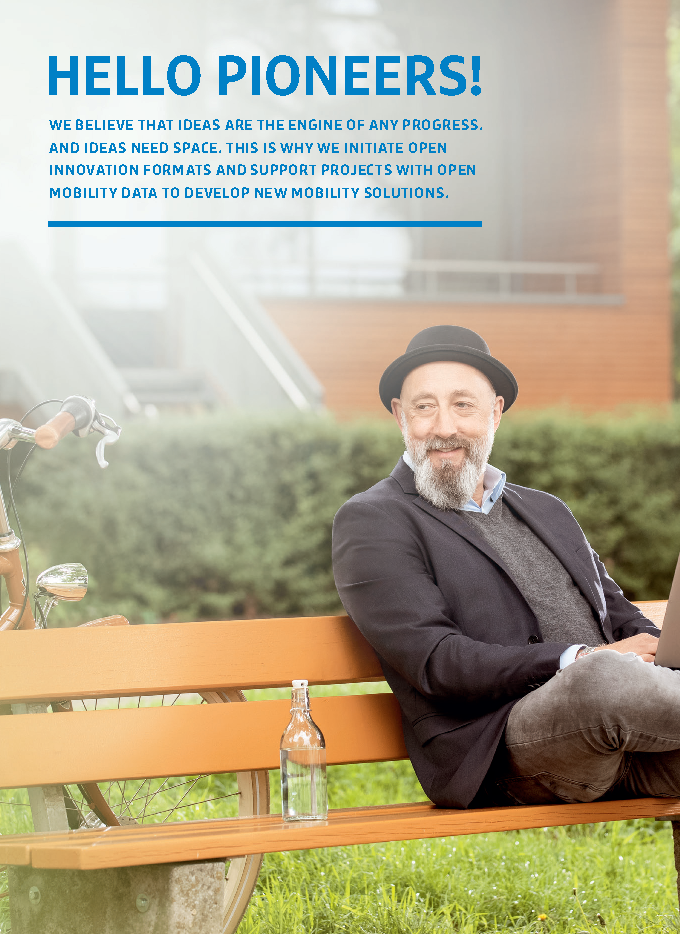
\includegraphics[pagebox=mediabox]{sponsors/ministerium-fuer-verkehr-left.pdf}%
  }%
]{mvleftadvertisement}
\newpairofpagestyles[]{sponsor-mvleft}{}
\AddLayersAtBeginOfPageStyle{sponsor-mvleft}{cropmarksplain}
\AddLayersAtBeginOfPageStyle{sponsor-mvleft}{mvleftadvertisement}

% Ministerium für Verkehr advertisement (right)
%TODO get rid of their cropmarks, add ours
\DeclareNewLayer[background,%
  width=115mm,%
  height=158mm,%
  hoffset=5mm,%
  voffset=5mm,%
  contents={%
    %TODO correct size
    
\includegraphics[pagebox=mediabox]{sponsors/ministerium-fuer-verkehr-right.pdf}%
  }%
]{mvrightadvertisement}
\newpairofpagestyles[]{sponsor-mvright}{}
\AddLayersAtBeginOfPageStyle{sponsor-mvright}{cropmarksplain}
\AddLayersAtBeginOfPageStyle{sponsor-mvright}{mvrightadvertisement}

% Geotab advertisement
\DeclareNewLayer[background,%
  width=125mm,%
  height=168mm,%
  hoffset=-0.4mm,%
  contents={%
    
\includegraphics{sponsors/geotab.pdf}%
  }%
]{geotabadvertisement}
\newpairofpagestyles[]{sponsor-geotab}{}
\AddLayersAtBeginOfPageStyle{sponsor-geotab}{geotabadvertisement}
\AddLayersAtBeginOfPageStyle{sponsor-geotab}{cropmarksplain}

% Grab advertisement
\DeclareNewLayer[background,%
  width=125mm,%
  height=168mm,%
  hoffset=-0.4mm,%
  contents={%
    
\includegraphics{sponsors/grab.pdf}%
  }%
]{grabadvertisement}
\newpairofpagestyles[]{sponsor-grab}{}
\AddLayersAtBeginOfPageStyle{sponsor-grab}{grabadvertisement}
\AddLayersAtBeginOfPageStyle{sponsor-grab}{cropmarksplain}

% Mapbox advertisement
\DeclareNewLayer[background,%
  width=125mm,%
  height=168mm,%
  contents={%
    
\includegraphics{sponsors/mapbox.pdf}%
  }%
]{mapboxadvertisement}
\newpairofpagestyles[]{sponsor-mapbox}{}
\AddLayersAtBeginOfPageStyle{sponsor-mapbox}{cropmarksplain}
\AddLayersAtBeginOfPageStyle{sponsor-mapbox}{mapboxadvertisement}

% Anyways advertisement
\DeclareNewLayer[background,%
  width=125mm,%
  height=168mm,%
  hoffset=-0.4mm,%
  contents={%
    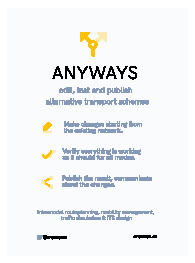
\includegraphics[width=125mm]{sponsors/anyways.pdf}%
  }%
]{anywaysadvertisement}
\newpairofpagestyles[]{sponsor-anyways}{}
\AddLayersAtBeginOfPageStyle{sponsor-anyways}{anywaysadvertisement}
\AddLayersAtBeginOfPageStyle{sponsor-anyways}{cropmarksplain}

% Telenav advertisement
\DeclareNewLayer[background,%
  width=125mm,%
  height=168mm,%
  hoffset=-0.4mm,%
  contents={%
    
\includegraphics[width=125mm]{sponsors/telenav.png}%
  }%
]{telenavadvertisement}
\newpairofpagestyles[]{sponsor-telenav}{}
\AddLayersAtBeginOfPageStyle{sponsor-telenav}{cropmarksplain}
\AddLayersAtBeginOfPageStyle{sponsor-telenav}{telenavadvertisement}

% OpenCage and Mapillary advertisement
\DeclareNewLayer[background,%
  width=115mm,%
  height=79mm,%
  hoffset=5mm,
  voffset=5mm,
  contents={%
    
\includegraphics[width=115mm, height=79mm]{sponsors/opencage.png}%
  }%
]{opencage}
\DeclareNewLayer[background,%
  width=115mm,%
  height=79mm,%
  hoffset=5mm,%
  voffset=84mm,%
  contents={%
    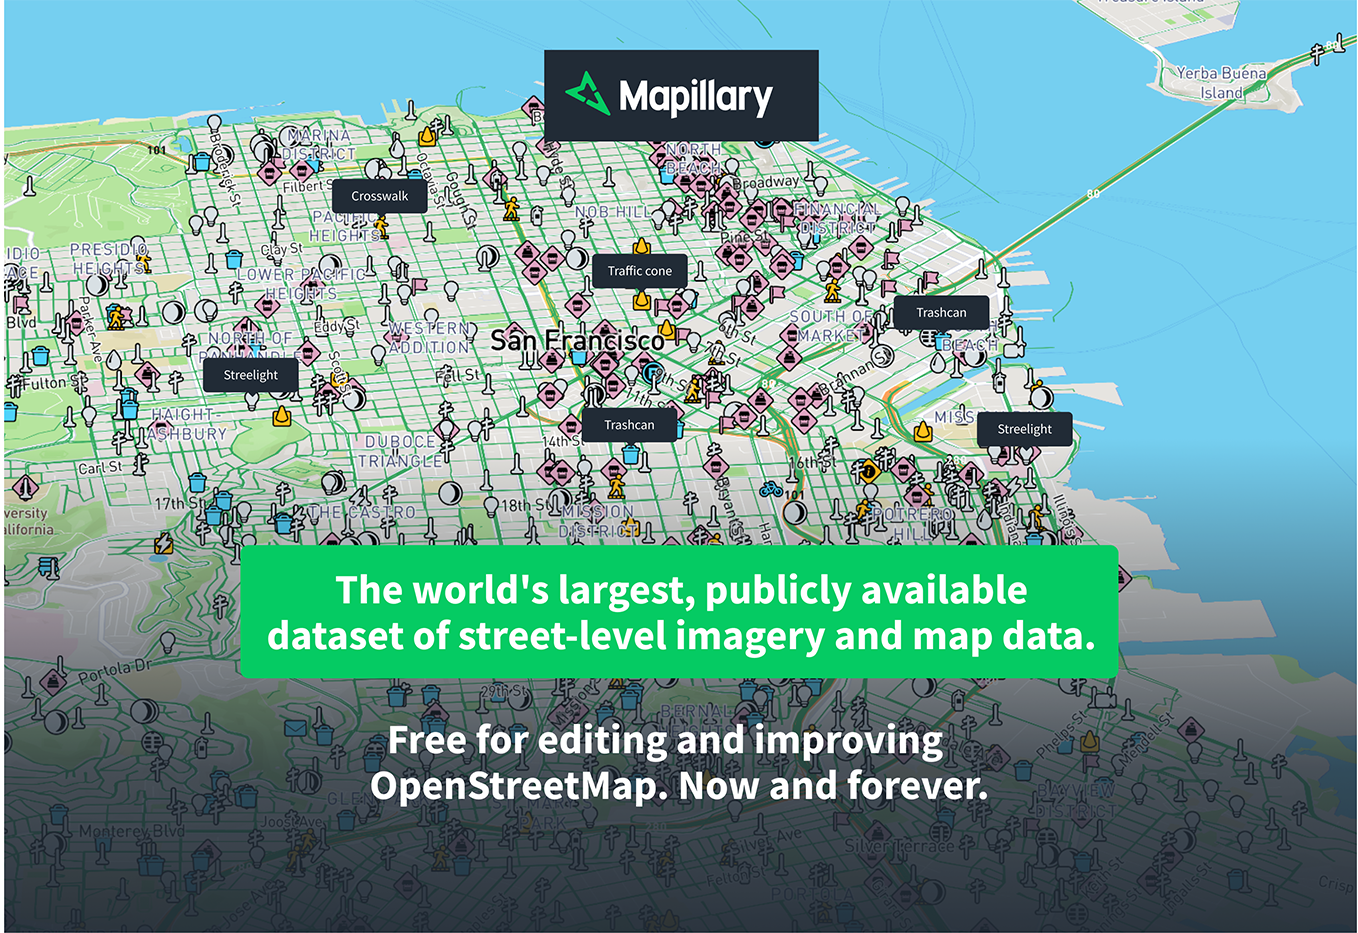
\includegraphics[width=115mm]{sponsors/mapillary.png}%
  }%
]{mapillary}
\newpairofpagestyles{sponsor-opencage-mapillary}{}
\AddLayersAtBeginOfPageStyle{sponsor-opencage-mapillary}{cropmarksevery}
\AddLayersAtBeginOfPageStyle{sponsor-opencage-mapillary}{opencage}
\AddLayersAtBeginOfPageStyle{sponsor-opencage-mapillary}{mapillary}

% IBM and OSADL advertisement
\DeclareNewLayer[background,%
  width=108mm,%
  height=77mm,%
  hoffset=8.5mm,
  voffset=7.0mm,
  contents={%
    
\includegraphics{sponsors/ibm.pdf}%
  }%
]{ibm}
\DeclareNewLayer[background,%
  width=115mm,%
  height=79mm,%
  hoffset=-0.4mm,%
  voffset=84mm,%
  contents={%
    
\includegraphics{sponsors/osadl.pdf}%
  }%
]{osadl}
\newpairofpagestyles{sponsor-ibm-osadl}{}
\AddLayersAtBeginOfPageStyle{sponsor-ibm-osadl}{ibm}
\AddLayersAtBeginOfPageStyle{sponsor-ibm-osadl}{osadl}
\AddLayersAtBeginOfPageStyle{sponsor-ibm-osadl}{cropmarksevery}

% Accenture and TomTom logo
\DeclareNewLayer[background,%
  width=84mm,%
  height=22.4mm,%
  hoffset=20mm,
  voffset=35mm,
  contents={%
    
\includegraphics[width=84mm]{sponsors/accenture.png}
  }%
]{accentureimage}
\DeclareNewLayer[background,%
  width=84mm,%
  height=25mm,%
  hoffset=18mm,
  voffset=104mm,
  contents={%
    
\includegraphics[width=97mm]{sponsors/tomtom.pdf}
  }%
]{tomtomimage}
\newpairofpagestyles[cropmarksstyle]{sponsor-accenture-tomtom}{}
\AddLayersAtBeginOfPageStyle{sponsor-accenture-tomtom}{accentureimage}
\AddLayersAtBeginOfPageStyle{sponsor-accenture-tomtom}{tomtomimage}
\AddLayersAtBeginOfPageStyle{sponsor-accenture-tomtom}{cropmarksevery}

% Facebook logo
\DeclareNewLayer[background,%
  width=83mm,%
  height=16mm,%
  hoffset=20mm,
  voffset=76mm,
  contents={%
    
\includegraphics[width=83mm]{sponsors/facebook.pdf}
  }%
]{facebookimage}
\newpairofpagestyles[cropmarksstyle]{sponsor-facebook}{}
\AddLayersAtBeginOfPageStyle{sponsor-facebook}{facebookimage}
\AddLayersAtBeginOfPageStyle{sponsor-facebook}{cropmarksevery}

% Bing logo
\DeclareNewLayer[background,%
  width=83mm,%
  height=16mm,%
  hoffset=20mm,
  voffset=67mm,
  contents={%
    
\includegraphics[width=83mm]{sponsors/bing.pdf}
  }%
]{bingimage}
\newpairofpagestyles[cropmarksstyle]{sponsor-bing}{}
\AddLayersAtEndOfPageStyle{sponsor-bing}{bingimage}
\AddLayersAtBeginOfPageStyle{sponsor-bing}{cropmarksevery}

% public transport map
\DeclareNewLayer[background,%
  width=105mm,%
  height=148mm,%
  hoffset=10mm,%
  voffset=10mm,%
  contents={%
    %TODO correct size
    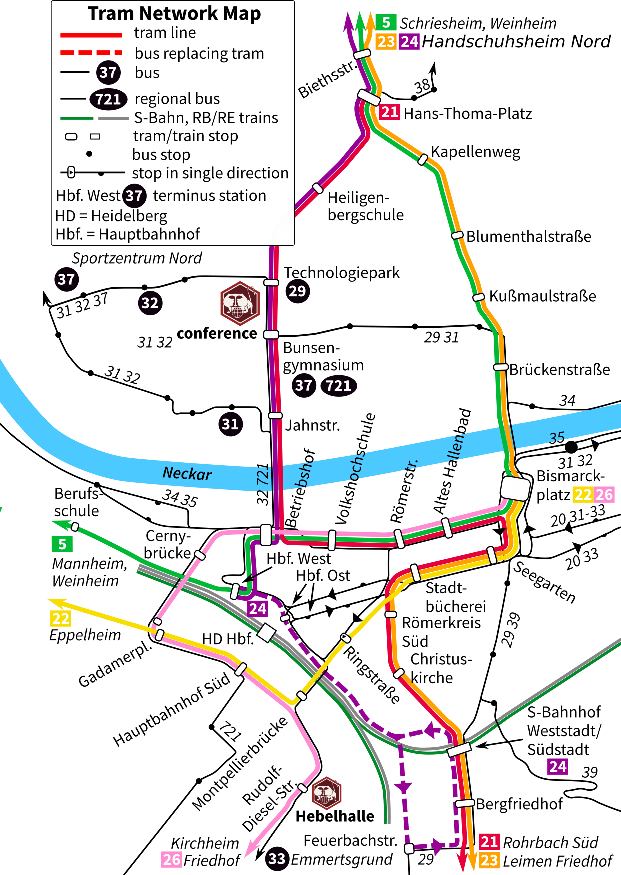
\includegraphics[]{images-print/public_transport.pdf}%
  }%
]{publictransport}
\newpairofpagestyles[]{page-public-transport}{}
\AddLayersAtBeginOfPageStyle{page-public-transport}{publictransport}
\AddLayersAtBeginOfPageStyle{page-public-transport}{cropmarksplain}

% city map
\definecolor{tram}{cmyk}{0 0 0 0.62}
\DeclareNewLayer[background,%
  width=115mm,%
  height=158mm,%
  hoffset=5mm,%
  voffset=5mm,%
  contents={%
    \begin{tikzpicture}[x=1mm, y=1mm]%
      % map image
      \draw (0,0) node [inner sep=0mm, anchor=south west] {%
        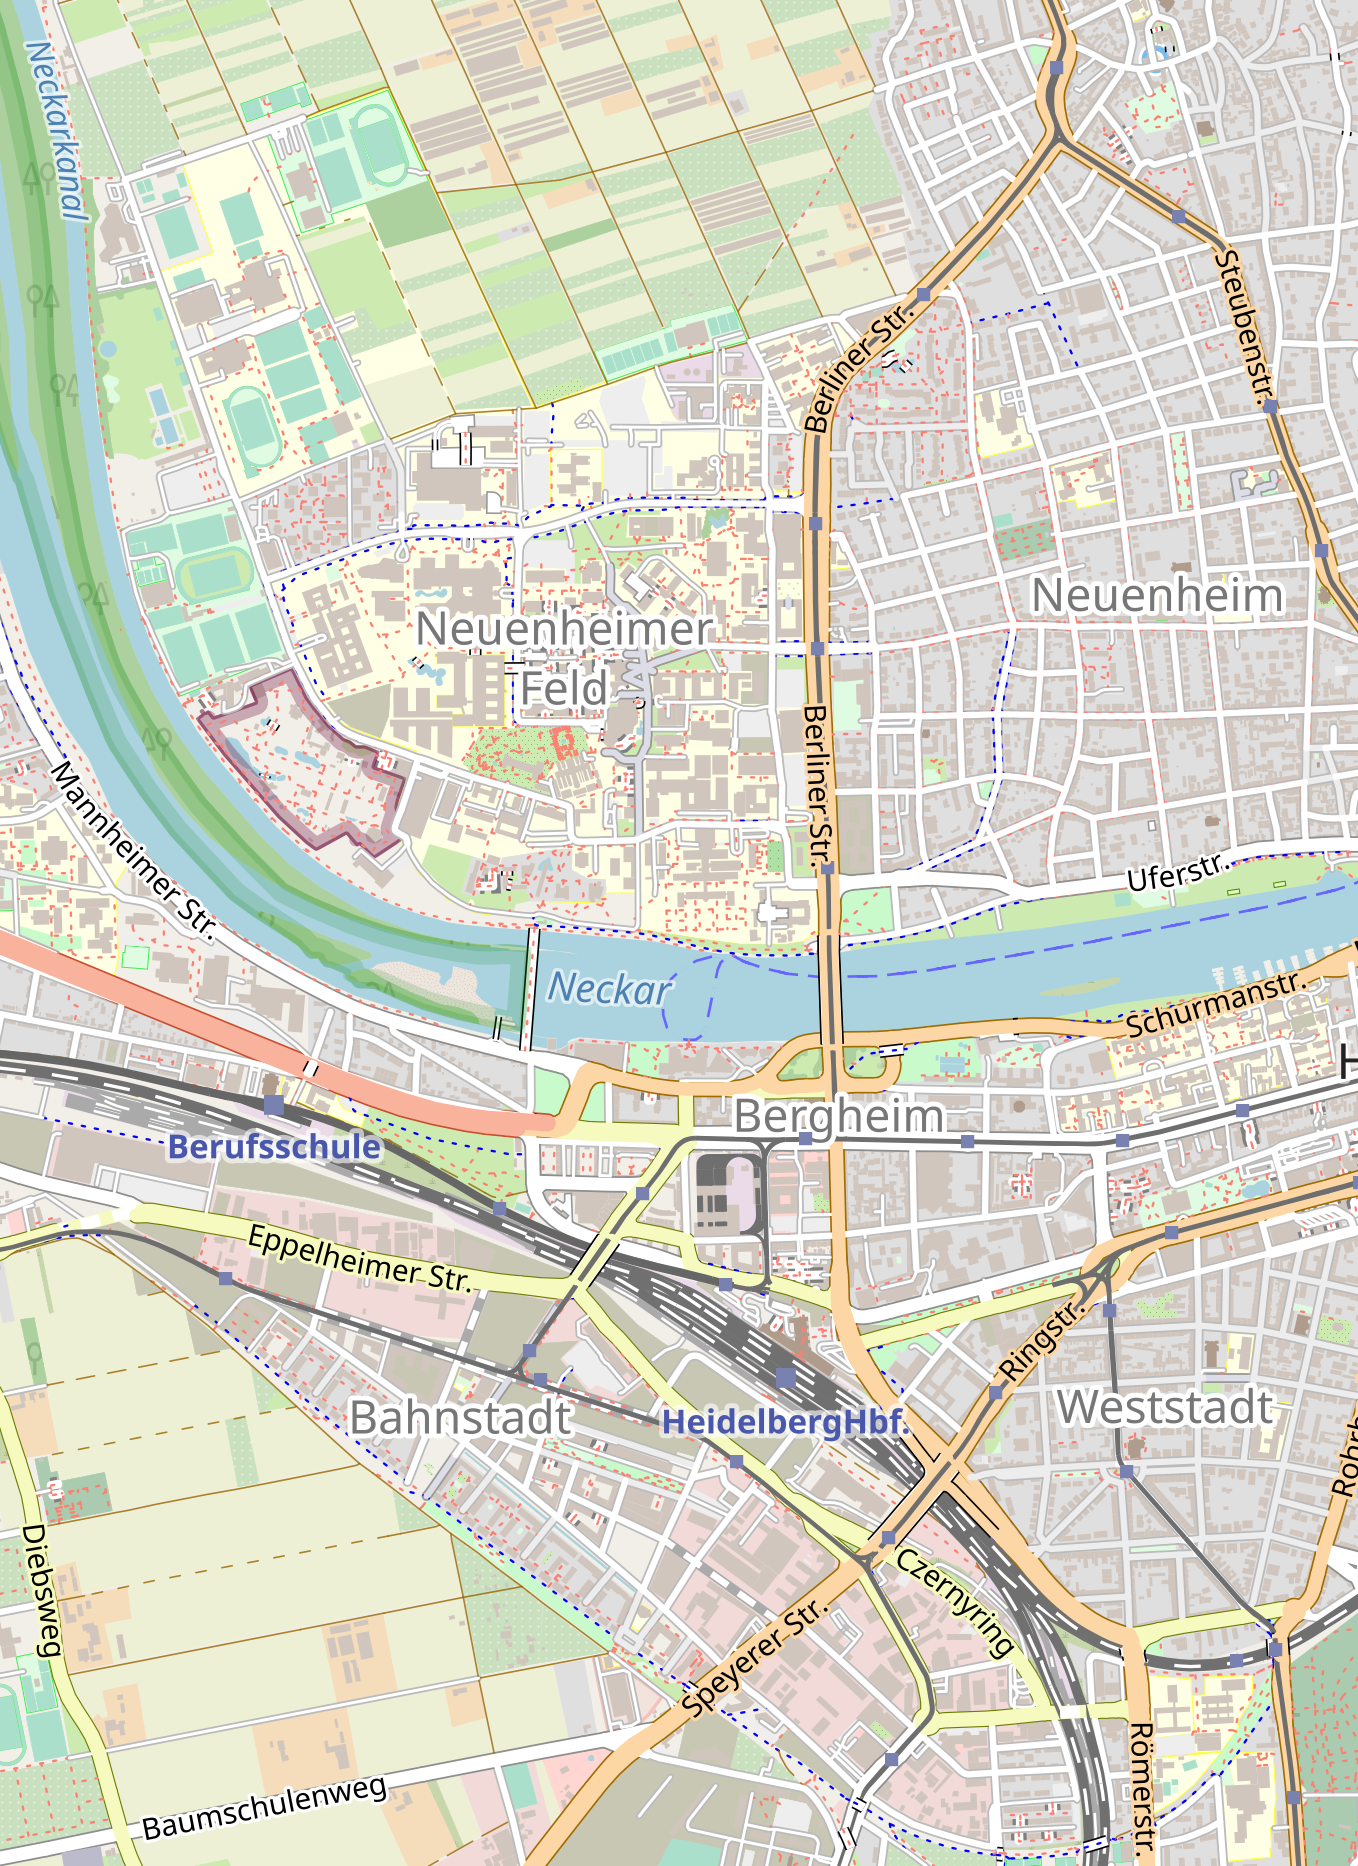
\includegraphics[width=115mm]{images-print/heidelberg-map-left.png}%
      };%
      % box for map key
      \fill [white] (0,32) rectangle (52,0);%
      % map key text
      \draw (8,8) node [anchor=south west, align=left] {%
        \begin{minipage}{47mm}%
          \small
          1 conference \hspace{1em}
          2 Botanic Garden \hspace{1em}\linebreak
          3 tram stop Hbf (since 2019-09-11) \hspace{1em}
          4 HebelHalle\hspace{1em}
          5 bridge closed \hspace{1em}\linebreak
          6 Philosophenweg \hspace{1em}\linebreak
          7 Old Bridge and monkey \hspace{1em}\linebreak
          8 Marstall \hspace{1em}
          9 castle
        \end{minipage}%
      };
      % tram line
      \draw [line width=0.33mm, color=tram] (64.95,48.95) -- (68.97,47.38) .. controls (70.63,46.87) and (72.80,45.17) .. (75.64,45.57) -- (89.85,49.39);
      \draw [line width=0.30mm, color=tram] (64.98,48.55) -- (68.92,46.98) .. controls (70.58,46.47) and (72.75,44.97) .. (75.64,45.57) -- (89.85,49.39);
      % circles with numbers
      \node (1) at (68.74,47.41) [] {}; % Hbf Nord
      \node (1label) at (1) [fill=white, draw=black, inner sep=0.3mm, circle] {\small 3}; % Hbf Nord (label)
      \node (2) at (90.6, 13.0) [] {}; % Hebelbrücke
      \node (2label) at (2) [fill=white, draw=black, inner sep=0.3mm, circle] {\small 5};
      \node (3) at (60.6, 110.5) [] {}; % Chemie-Hörsaalgebäude
      \node (3label) at (3) [fill=white, draw=black, inner sep=0.3mm, circle] {\small 1}; % Chemie-Hörsaalgebäude
      \node (4) at (78.31, 9.02) [] {}; % Hebelhalle
      \node (4label) at (4) [fill=white, draw=black, inner sep=0.3mm, circle] {\small 4};
      \node (5) at (43.3, 93.8) [] {}; % Botanischer Garten
      \node (5label) at (5) [fill=white, draw=black, inner sep=0.3mm, circle] {\small 2}; % Botanischer Garten
    \end{tikzpicture}%
  }%
]{citymapleft}
\newpairofpagestyles[]{page-citymap-left}{}
\AddLayersAtBeginOfPageStyle{page-citymap-left}{citymapleft}
\AddLayersAtBeginOfPageStyle{page-citymap-left}{cropmarksplain}
\DeclareNewLayer[background,%
  width=115mm,%
  height=158mm,%
  hoffset=5mm,%
  voffset=5mm,%
  contents={%
    \begin{tikzpicture}[x=1mm, y=1mm]%
      % node for extend
      % map image
      \draw (0,0) node [inner sep=0mm, anchor=south west] {%
        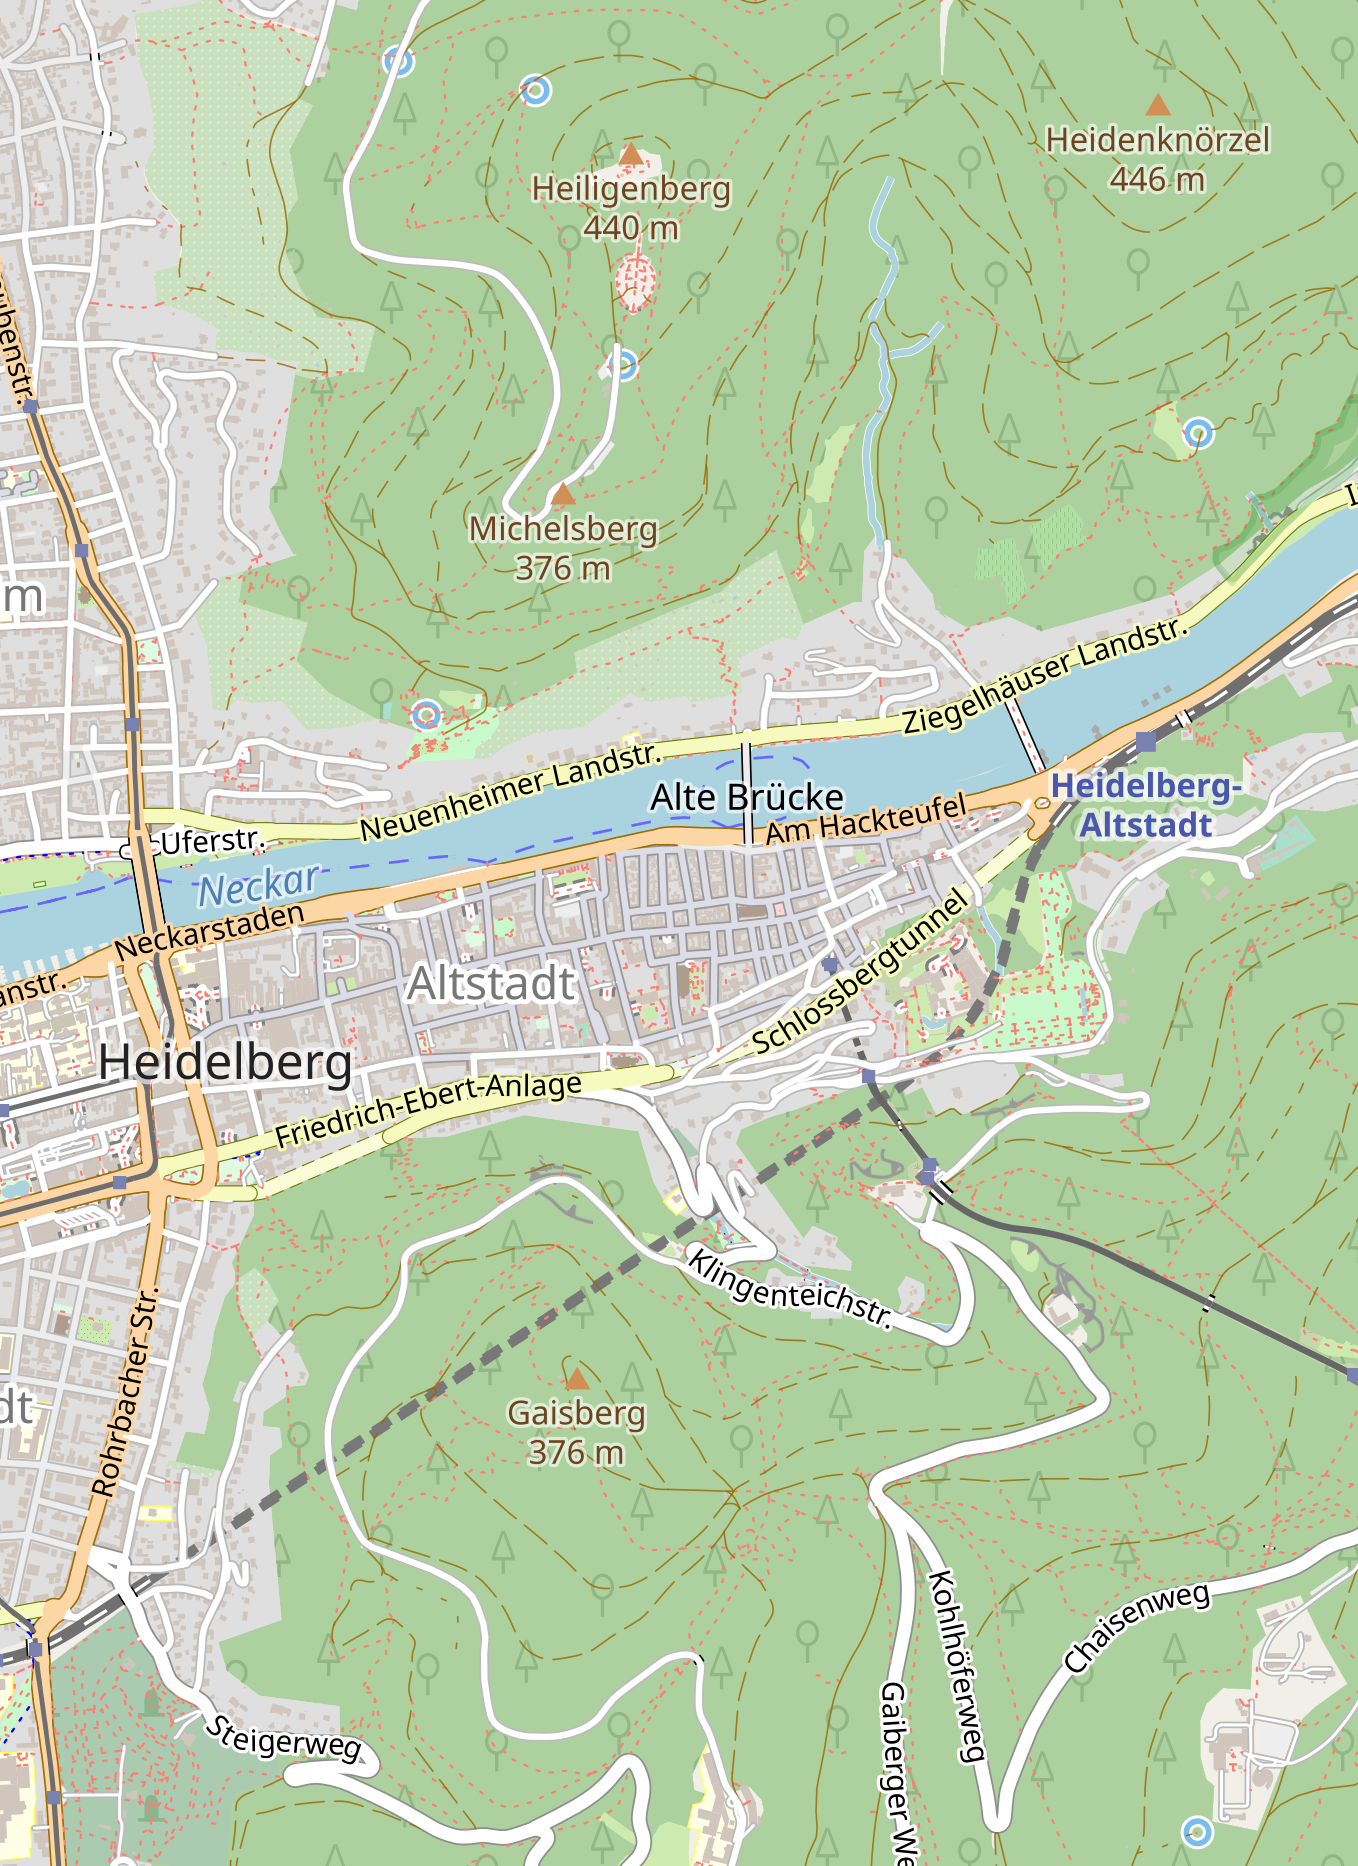
\includegraphics[width=115mm]{images-print/heidelberg-map-right.png}%
      };%
      % circles with numbers
      \node (6) at (55.4, 103.3) [] {}; % Philosophenweg
      \node (6label) at (6) [fill=white, draw=black, inner sep=0.3mm, circle] {\small 6};
      \node (7) at (81.3, 74.9) [] {}; % castle
      \node (7label) at (7) [fill=white, draw=black, inner sep=0.3mm, circle] {\small 9};
      \node (8) at (62.9, 87.7) [] {}; % Old Bridge
      \node (8label) at (8) [fill=white, draw=black, inner sep=0.3mm, circle] {\small 7};
      \node (9) at (48.1, 84.46) [] {}; % Old Bridge
      \node (9label) at (9) [fill=white, draw=black, inner sep=0.3mm, circle] {\small 8};
    \end{tikzpicture}%
  }%
]{citymapright}
\newpairofpagestyles[]{page-citymap-right}{}
\AddLayersAtBeginOfPageStyle{page-citymap-right}{citymapright}
\AddLayersAtBeginOfPageStyle{page-citymap-right}{cropmarksplain}

% campus map
\DeclareNewLayer[background,%
  width=115mm,%
  height=158mm,%
  hoffset=5mm,%
  voffset=5mm,%
  contents={%
    %TODO correct size
    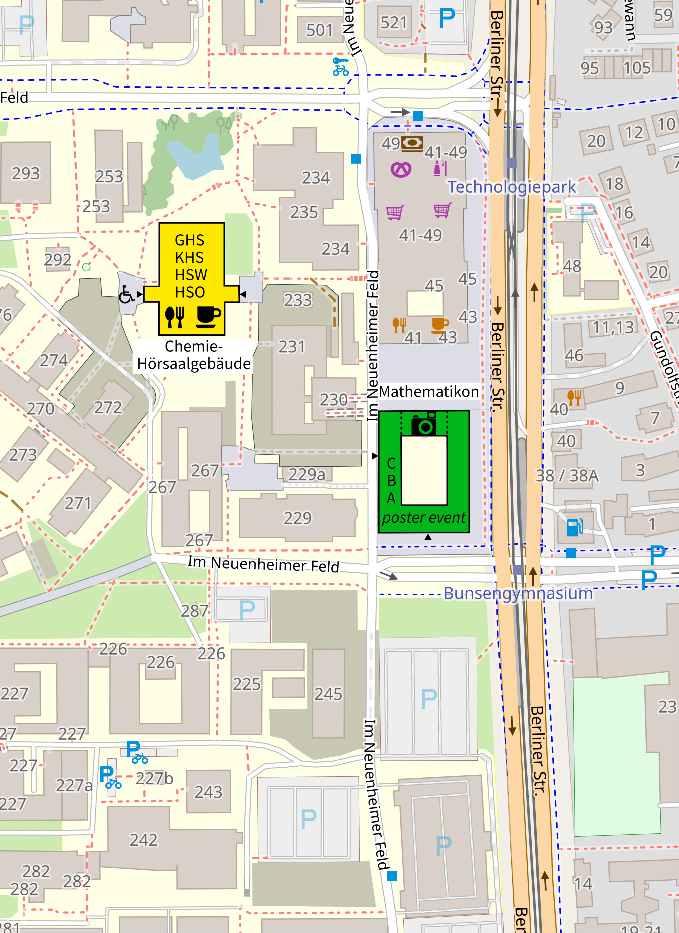
\includegraphics[]{images-print/campus.pdf}%
  }%
]{campus}
\newpairofpagestyles[]{page-campus}{}
\AddLayersAtBeginOfPageStyle{page-campus}{campus}
\AddLayersAtBeginOfPageStyle{page-campus}{cropmarksplain}


\begin{document}

% color of table rules
\taburulecolor{tableRuleGray}
 
%\pagestyle{cropmarksstyle}
\begin{titlepage}
  \thispagestyle{titlestyle}
  \null
\end{titlepage}
\pagestyle{cropmarksstyle}

\selectlanguage{english}
\section*{Content}
\newlength\contentspace
\setlength\contentspace{\contentspace}

\vspace*{\contentspace}%
\noindent Welcome\dotfill \pageref{welcome}
%
%\vspace*{\contentspace}%
%\noindent Scholarships \dotfill \pageref{scholarships}
%
%\vspace*{\contentspace}%
%\noindent Getting around in Milan \dotfill \pageref{getting-around}
%
%\vspace*{\contentspace}%
%\noindent Code of Conduct \dotfill \pageref{coc}

\vspace*{\contentspace}%
\noindent Saturday schedule \dotfill \pageref{saturday}

\vspace*{\contentspace}%
\noindent Social Event \dotfill \pageref{social-event}

\vspace*{\contentspace}%
\noindent Sunday schedule \dotfill \pageref{sunday}

\vspace*{\contentspace}%
\noindent Monday schedule \dotfill \pageref{monday}

\vspace*{\contentspace}%
\noindent Saturday \dotfill \pageref{saturday-descriptions}

\vspace*{\contentspace}%
\noindent Sunday \dotfill \pageref{sunday-descriptions}

\vspace*{\contentspace}%
\noindent Monday \dotfill \pageref{monday-descriptions}

\vspace*{\contentspace}%
\noindent Thanks \dotfill \pageref{thanks}

\vspace*{\contentspace}%
\noindent Sponsors \dotfill \pageref{sponsors}
%
%\vspace*{\contentspace}%
%\noindent Maps \dotfill \pageref{maps}

\vspace*{\contentspace}%
\noindent Legal notice \dotfill \pageref{legal}

\vfill
\noindent
Hashtag: \#sotm

\vspace*{0.8em}%
\noindent
The general emergency telephone number in Germany is \textbf{112}.
\vfill

\small{
\noindent
  \** Sessions in this room will not be recorded on video.\\
  \**\** This session will not be recorded on video.\\
  \diamondSymbol\ The title of this talk is not provided in full length in the schedule table. Please refer to the short description at pages \ref{abstracts}~et seqq. for the full title and list of authors.
}\normalsize


\newpage

\newpage
\enlargethispage{1\baselineskip}
\section*{Welcome to Heidelberg and State of the Map 2019} \label{welcome}
This booklet provides you essential information
about the conference, the location and the schedule.  We are proud of the participation of the
OpenStreetMap community and our rich program but there is even more!  Please do get involved and
take advantage of the off-schedule sessions, discussions and spaces.

\paragraph*{Help desk} \label{welcome-helpdesk}
You already know the help desk, located on the ground floor of the Chemie-Hörsaalgebäude (Chemistry
Lecture Halls Building). It is also your port of call if you need support or help.

\paragraph*{Programme}
You can find the diverse programme on page~\pageref{saturday}f. Full abstracts of all talks are
available at https://2019.stateofthe\\map.org/program for the general tracks and
https://2019.stateofthemap.org/academic\_programme for the academic track.

\paragraph*{Self-organised sessions} \label{welcome-location}
Rooms A, B and C in the Mathematikon building are available for self-organised sessions if they are not in use by pre-schedule sessions (see this booklet). Please come to the help desk in the Chemie-Hörsaalgebäude to announce your session.

\paragraph*{Sponsors} \label{welcome-sponsors}
We would like to thank our sponsors for making this event possible and for their support to the
OpenStreetMap Foundation.
\newpage

\newpage
\small
\renewcommand{\arraystretch}{1.4}
%\section*{Saturday Schedule}
\label{saturday}
\pagestyle{saturday-table}
\setPageBackground
\noindent\begin{landscape}
  \begin{center}
    \noindent\begin{tabular}{Z{0.75cm}Z{2.38cm};{0.2mm/2mm}Z{2.38cm};{0.2mm/2mm}Z{2.38cm};{0.2mm/2mm}Z{2.38cm};{0.2mm/2mm}}
      \cellcolor{commongray}
      &
      \multicolumn{4}{c}{
        \cellcolor{GHS}
        GHS
      }
      \tabularnewline
      \cellcolor{commongray}
      09:30
      \multiColTalk{4}{Z{9.52cm}}{Welcome}{}
      \tabularnewline
      \programHRule{5}
      \cellcolor{commongray}
      10:00
      \multiColTalk{4}{Z{9.52cm}}{\emph{Keynote} Open up! Why digital mobility needs participation}{Christian Förster, Dietmar Seifert}
      \tabularnewline
      \programHRule{5}
      \cellcolor{commongray}
      10:30
      \multiColTalk{4}{Z{9.52cm}}{\emph{Keynote}}{Karen Sandler}
      \tabularnewline
      \rowcolor{commongray}
      11:00
      & \multicolumn{4}{c}{%
      \parbox[c]{24pt}{%
        
\includegraphics[height=10pt]{cafe}%
      }
      break}
      \tabularnewline
      \cellcolor{commongray}
      & \multicolumn{1}{c}{\cellcolor{GHS} GHS}
      & \multicolumn{1}{c}{\cellcolor{HSO} HSO}
      & \multicolumn{1}{c}{\cellcolor{HSW} HSW}
      & \multicolumn{1}{c}{\cellcolor{KHS} KHS*}
      \tabularnewline
      \cellcolor{commongray}
      11:30
      \talk{Get to know OSGeo and how OSGeo is connected to OSM}{Astrid Emde}
      \talk{Data Quality and Feature Extraction at scale with RoboSat.pink}{Oliver Courtin}
      \longTalk{2}{Introduction to OSM: How it's made and how it's used}{Thomas Skowron, Frederik Ramm}
      \longTalk{2}{\emph{Workshop}\linebreak Mapping public transport and cycling itineraries using JOSM's PT\_Assistant plugin}{Polyglot}
      \tabularnewline
      \programCRule{2-3}
      \cellcolor{commongray}
      12:00
      \talk{``Keepin' it fresh (and good)!''\,\diamondSymbol}{Kevin Ventullo, Christopher Klaiber}
      \talk{Human Mapping with Machine Data}{Christopher Beddow, Edoardo Neerhut}
      &
      &
      \tabularnewline
      \programCRule{2-3}
      \programCRule{5-5}
    \end{tabular}
    \newpage

    \noindent\begin{tabular}{Z{0.75cm}Z{2.38cm};{0.2mm/2mm}Z{2.38cm};{0.2mm/2mm}Z{2.38cm};{0.2mm/2mm}Z{2.38cm};{0.2mm/2mm}}
      \cellcolor{commongray}
      & \multicolumn{1}{c}{\cellcolor{GHS} GHS}
      & \multicolumn{1}{c}{\cellcolor{HSO} HSO}
      & \multicolumn{1}{c}{\cellcolor{HSW} HSW}
      & \multicolumn{1}{c}{\cellcolor{KHS} KHS*}
      \tabularnewline
      \cellcolor{commongray}
      12:30
      \talk{Driving South East Asia Forward with OpenStreetMap}{Jinal Foflia}
      \talk{Assisted Intelligence~-- How we map with the support of new technologies}{Felix Delattre, Surabhi Singh}
      &
      &
      \tabularnewline
      \rowcolor{commongray}
      13:00
      & \multicolumn{4}{c}{%
      \parbox[c]{24pt}{%
        
\includegraphics[height=10pt]{restaurant}%
      }
      lunch}
      \tabularnewline
      \cellcolor{commongray}
      14:00
      \talk{ODbL license compatibility}{Kathleen Lu}
      \talk{Lightning Talks I}{}
      \longTalk{2}{Share Edits and Insights with the Overpass Tools}{Roland Olbricht}
      \longTalk{2}{\emph{Workshop}\linebreak How to contribute to weeklyOSM via the CMS: OSMBC}{Manfred Reiter}
      \tabularnewline
      \programCRule{2-3}
      \cellcolor{commongray}
      14:30
      \talk{Communication and Knowledge Transfer in OSM}{Hanna Krüger}
      \talk{OsmInEdit~-- a simple indoor editor}{Adrien Pavie et\,al.}
      &
      &
      \tabularnewline
      \programHRule{5}
      \cellcolor{commongray}
      15:00
      \talk{Past and Future of the OSMF Membership Working Group}{Michael Spreng}
      \talk{Observe~-- offline, cross-platform field mapping tool for OpenStreetMap}{Sajjad Anwar}
      &
      &
      \tabularnewline
      \programHRule{5}
    \end{tabular}
    \newpage

    \noindent\begin{tabular}{Z{0.75cm}Z{2.38cm};{0.2mm/2mm}Z{2.38cm};{0.2mm/2mm}Z{2.38cm};{0.2mm/2mm}Z{2.38cm};{0.2mm/2mm}}
      \cellcolor{commongray}
      & \multicolumn{1}{c}{\cellcolor{GHS} GHS}
      & \multicolumn{1}{c}{\cellcolor{HSO} HSO}
      & \multicolumn{1}{c}{\cellcolor{HSW} HSW}
      & \multicolumn{1}{c}{\cellcolor{KHS} KHS*}
      \tabularnewline
      \rowcolor{commongray}
      15:30
      & \multicolumn{4}{c}{%
      \parbox[c]{24pt}{%
        
\includegraphics[height=10pt]{photo}%
      }
      photo (courtyard of Mathematikon building)}
      \tabularnewline
      \rowcolor{commongray}
      16:00
      & \multicolumn{4}{c}{%
        \parbox[c]{24pt}{%
          
\includegraphics[height=10pt]{cafe}%
        }
      break}
      \tabularnewline
      \cellcolor{commongray}
      16:30
      \talk{OSM Data: From Digital to Physical Design}{Yantisa Akhadi}
      \talk{Lightning Talks II}{}
      \longTalk{2}{Board and working groups meeting \emph{(public)}}{}
      \longTalk{2}{\emph{Workshop}\linebreak uMap for newbies}{Manfred Reiter}
      \tabularnewline
      \programCRule{2-3}
      \cellcolor{commongray}
      17:00
      \talk{CyclOSM, a bicycle oriented render for every cyclist}{Lucas Verney, Florimond Berthoux}
      \talk{VR Map: Using OSM Data In a WebVR Environment}{Robert Kaiser}
      &
      &
      \tabularnewline
      \programCRule{2-3}
      \programCRule{5-5}
      \cellcolor{commongray}
      17:30
      \talk{How to use OSM data with the Desktop GIS QGIS}{Astrid Emde}
      \talk{Hikar~-- OSM Augmented Reality for Walkers across Europe}{Nick Whitelegg}
      &
      &
      \tabularnewline
      \programHRule{5}
    \end{tabular}
    \newpage

    \label{social-event}%
    \enlargethispage{1\baselineskip}%
    \newlength\socialEventBoxWidth
    \setlength{\socialEventBoxWidth}{10.82cm}
    \newlength\socialEventSectionSep
    \setlength{\socialEventSectionSep}{\baselineskip}
    \noindent\begin{tabular}{Z{0.75cm}Z{\socialEventBoxWidth};{0.2mm/2mm}}
      \rowcolor{ochsenblutrot}
      \parbox[t]{\linewidth}{%
        \textcolor{white}{19:00}%
      }%
      &
      \multicolumn{1}{C{\socialEventBoxWidth}}{%
        \textcolor{white}{%
          Social Event at Hebelhalle
        }%
      }
      \tabularnewline
      \cellcolor{ochsenblutrot}
      &
      \begin{minipage}[t]{\socialEventBoxWidth}
        \noindent\begin{minipage}[t]{0.47\linewidth}
          \vspace{-0.56\baselineskip}
          \begin{wrapfigure}[6]{r}[0pt]{0.4\linewidth}%
            \vspace{-1\baselineskip}%
            \qrcode[height=18mm,padding]{geo:49.39655,8.67945}%
          \end{wrapfigure}%
          \textbf{Location}\\
          Hebelhalle\\
          Hebelstraße 9\\
          69115 Heidelberg\\
          geo:49.39655,8.67945\\
          entrance from Gottlieb-Daimler-Straße

          \vspace{\socialEventSectionSep}
          \textbf{Getting there by public transport}\\
          next tram stop: Rudolf-Diesel-Straße\\
          tram line 26, bus line 33

          \vspace{\socialEventSectionSep}
          \textbf{Programme}\\
          Welcome\\
          Dinner and music\\
          OSM Awards ceremony

          \vspace{\baselineskip}
          Catering is provide by a local catering company employing refugees from Syria.
        \end{minipage}
        \hfill
        \noindent\begin{minipage}[t]{0.47\linewidth}
          \begin{center}
            \noindent tabbouleh salad with fried shrimps\\
            $\blackdiamond$\\
            couscous salad with fried vegetables and herbs\\
            $\blackdiamond$\\
            baguette with hummus and sprouts and dried tomatoes\\
            $\blackdiamond$\\
            fresh figs and prickly pears with balsamic reduction, soft goats cheese, ham and bread\\
            $\blackdiamond$\\
            stewed beef in orange, cocos and fresh coriander sauce, rice\\
            $\blackdiamond$\\
            Syrian dal from lentils with lime, spices, fresh herbs, cocos milk and pumpkin topping, rice\\
            $\blackdiamond$\\
            desserts

            \noindent \emph{The menu might be subject of change.}
          \end{center}
        \end{minipage}
      \end{minipage}
      \vspace{0.4\multicolsep}
      \tabularnewline
      \programHRule{2}
    \end{tabular}
  \end{center}
  \newpage
\end{landscape}
\renewcommand{\arraystretch}{1.0}

\newpage
\renewcommand{\arraystretch}{1.4}
%\section*{Sunday Schedule}
\label{sunday}
\pagestyle{sunday-table}
\setPageBackground
\noindent\begin{landscape}
  \begin{center}
    \enlargethispage{1\baselineskip}
    \noindent\begin{tabular}{Z{0.75cm}Z{2.18cm}|Z{2.38cm}|Z{3.26cm}|Z{1.7cm}|}
      \cellcolor{table-header}
      &
      \multicolumn{4}{c}{
        \tableColHead{Hörsaal West}
      }
      \tabularnewline
      \cellcolor{table-header}
      09:00
      &
      \multicolumn{4}{Z{9.7cm}|}{%
        \textbf{Bridging the Map? Exploring Interactions between the Academic and Mapping Communities in OSM}
        % no newline to save space
        \hspace{1em}
        \emph{A. Yair Grinberger et\,al.}%
      }
      \tabularnewline
      \cellcolor{table-header}
      & \multicolumn{1}{c}{\tableColHead{Großer Hörsaal}}
      & \multicolumn{1}{c}{\tableColHead{Hörsaal Ost}}
      & \multicolumn{1}{c}{\tableColHead{Hörsaal West}}
      & \multicolumn{1}{c}{\tableColHead{KHS~\noVideo}}
      \tabularnewline
      \tableRowFirstCell{09:30}
      \talk{Flexible Routing with Graph\-Hopper}{Peter Karich}
      \talk{``Mapathon, Mapathon, Mapathon!''}{Séverin Menard, Nicolas Chavent}
      \talk{OpenStreetMap as a Space~\noVideo}{Dipto Sarkar, So Hoi Kay}
      \longTalk{3}{Scholar\linebreak Lightning\linebreak Talks}{}
      \tabularnewline
      \programHRule{4}
      \tableRowFirstCell{10:00}
      \talk{Imagery\linebreak Solutions in OSM}{Kevin Bullock}
      \talk{Associations Dynamics in French Speaking Africa\,\diamondSymbol}{Séverin Menard, Nicolas Chavent}
      \talk{Analysis of OSM Data through OSM Notes User Posting}{Toshikazu Seto et\,al.}
      &
      \tabularnewline
      \programHRule{4}
      \tableRowFirstCell{10:30}
      \talk{Lightning\linebreak Talks III}{}
      \talk{Tales from the Tasking Manager}{Ramya Ragupathy et\,al.}
      \talkSingleLine{A Novel Application of Models of Species Abundance to Better Understand OSM Community Structure and Interactions}{P. Mooney}
      &
      \tabularnewline
      \programHRule{5}
    \end{tabular}
  \end{center}
  \newpage

  \begin{center}
    \noindent\begin{tabular}{Z{0.75cm}Z{1.80cm}|Z{1.80cm}|Z{2.60cm}|Z{1.40cm}|Z{1.50cm}|}
      \cellcolor{table-header}
      & \multicolumn{1}{c}{\tableColHead{Großer Hörsaal}}
      & \multicolumn{1}{c}{\tableColHead{Hörsaal Ost}}
      & \multicolumn{1}{c}{\tableColHead{Hörsaal West}}
      & \multicolumn{1}{c}{\tableColHead{KHS~\noVideo}}
      & \multicolumn{1}{c}{\tableColHead{Math. C~\noVideo}}
      \tabularnewline
      \tableRowFirstCell{11:00}
      &
      \multicolumn{5}{c}{%
        \cellcolor{commongray}
        \parbox[c]{24pt}{%
          
\includegraphics[height=10pt]{cafe}%
        }%
        Break%
      }
      \tabularnewline
      \tableRowFirstCell{11:30}
      \talk{Overview of Map Serving Architectures}{Paul Norman}
      \talk{Our Falkirk~-- Mitigating the Impacts of Poverty\,\diamondSymbol}{Alison Moon}
      \talk{Towards Scalable Geospatial Remote Sensing for Efficient OSM Labeling\,~\noVideo}{Rui Zhang et\,al.}
      \longTalk{3}{Bilingual Breakout Session}{Séverin Menard, Nicolas Chavent}
      \longTalk{2}{\emph{Workshop}\linebreak First steps with OSM\linebreak Editors}{Angjelina Dervishaj}
      \tabularnewline
      \programCRule{2-4}
      \tableRowFirstCell{12:00}
      \talk{Customising Search for Special-Interest Maps}{S. Hoffmann}
      \talk{Metrics to Monitor\linebreak Buildings\linebreak Outbounds\,\diamondSymbol}{Pierre Béland}
      \talk{Estimating Latent Energy Demand of Buildings}{Nikola Milojevic-Dupont et\,al.}
      &
      &
      \tabularnewline
      \programCRule{2-4}
      \programCRule{6-6}
      \tableRowFirstCell{12:30}
      \talk{Is Your OSM App Spying on You?}{Thomas Skowron}
      \talk{Integrating Quality Assurance Checks into Map \mbox{Editors}\,\diamondSymbol}{David Manzer et\,al.}
      \talk{Client-Side Route Planning: Preprocessing the OSM Road Network for Routable Tiles}{Harm Delva et\,al.}
      &
      &
      \tabularnewline
      \programHRule{6}
    \end{tabular}
  \end{center}
  \newpage

  \begin{center}
    \noindent\begin{tabular}{Z{0.75cm}Z{2.00cm}|Z{1.80cm}|Z{2.30cm}|Z{1.50cm}|Z{1.60cm}|}
      \cellcolor{table-header}
      & \multicolumn{1}{c}{\tableColHead{Großer Hörsaal}}
      & \multicolumn{1}{c}{\tableColHead{Hörsaal Ost}}
      & \multicolumn{1}{c}{\tableColHead{Hörsaal West}}
      & \multicolumn{1}{c}{\tableColHead{KHS~\noVideo}}
      & \multicolumn{1}{c}{\tableColHead{Math. C~\noVideo}}
      \tabularnewline
      \rowcolor{commongray}
      \tableRowFirstCell{13:00}
      &
      \multicolumn{5}{c}{%
        \cellcolor{commongray}
        \parbox[c]{24pt}{%
          
\includegraphics[height=10pt]{restaurant}%
        }%
        Lunch%
      }
      \tabularnewline
      \tableRowFirstCell{14:00}
      \talk{What's behind JOSM?}{Vincent Privat}
      \talk{Spatial Indexes for OSM in PostGIS}{Felix Kunde}
      \talk{Intrinsic Assessment of Contri\-bution Patterns through Explora\-tory Spatial Data Analysis}{Marco Minghini et\,al.}
      \longTalk{2}{Diversity and Inclusion in OSM}{Patricia Solis et\,al.}
      \longTalk{2}{\emph{Workshop}\linebreak Using \mbox{OSMCha} to Understand Bad Edits}{Andrey Golovin et\,al.}
      \tabularnewline
      \programCRule{2-4}
      \tableRowFirstCell{14:30}
      \talk{Mapping Solar Panels Can Save Megatons of CO\textsubscript{2}}{Dan Stowell, Jerry Clough}
      \talk{Lightning Talks IV}{}
      \talk{Corporate Editors in the Evolving Landscape of OSM: A Close Investigation of the Impact to the Map and Community}{Jennings Anderson et\,al.}
      &
      &
      \tabularnewline
      \programHRule{6}
    \end{tabular}
  \end{center}
  \newpage

  \begin{center}
    \noindent\begin{tabular}{Z{0.75cm}Z{2.00cm}|Z{1.80cm}|Z{2.30cm}|Z{1.50cm}|Z{1.60cm}|}
      \cellcolor{table-header}
      & \multicolumn{1}{c}{\tableColHead{Großer Hörsaal}}
      & \multicolumn{1}{c}{\tableColHead{Hörsaal Ost}}
      & \multicolumn{1}{c}{\tableColHead{Hörsaal West}}
      & \multicolumn{1}{c}{\tableColHead{KHS~\noVideo}}
      & \multicolumn{1}{c}{\tableColHead{Math. C~\noVideo}}
      \tabularnewline
      \tableRowFirstCell{15:00}
      \talk{National Trust~-- Managing a Path Inventory in OSM: Towards an Open Paths Standard in OSM for the UK}{Huw Davies}
      \longTalk{2}{OSM Data Processing with PostgreSQL/\allowbreak PostGIS}{Jochen Topf}
      \talk{Exploring the \mbox{Effects} of Pokémon Go Vandalism on OSM}{Levente Juhász et\,al.}
      \longTalk{2}{Nomad Maps, an Andean Cartographic Itinerancy by Bike \emph{(Video)}}{Alban Vivert}
      \bookableSpace
      \tabularnewline
      \programCRule{2-2}
      \programCRule{4-4}
      \programCRule{6-6}
      \tableRowFirstCell{15:30}
      \talk{Collaborative Mapping of Cycling Infrastructure for Route and Thematic Maps~\diamondSymbol}{Carolina Ortega Espinosa}
      &
      \talk{Analysing the Spatio-Temporal Patterns and Impacts of Large-Scale Data Production Events in OSM}{A. Yair Grinberger et\,al.}
      &
      \bookableSpace
      \tabularnewline
      \tableRowFirstCell{16:00}
      &
      \multicolumn{5}{c}{%
        \cellcolor{commongray}
        \parbox[c]{24pt}{%
          
\includegraphics[height=10pt]{cafe}%
        }%
        Break%
      }
      \tabularnewline
    \end{tabular}
  \end{center}
  \newpage

  \begin{center}
    \noindent\begin{tabular}{Z{0.75cm}Z{2.20cm}|Z{1.30cm}|Z{2.70cm}|Z{1.40cm}|Z{1.60cm}|}
      \cellcolor{table-header}
      & \multicolumn{1}{c}{\tableColHead{Großer Hörsaal}}
      & \multicolumn{1}{c}{\tableColHead{Hörsaal Ost}}
      & \multicolumn{1}{c}{\tableColHead{Hörsaal West}}
      & \multicolumn{1}{c}{\tableColHead{KHS~\noVideo}}
      & \multicolumn{1}{c}{\tableColHead{Math. C~\noVideo}}
      \tabularnewline
      \tableRowFirstCell{16:30}
      \talk{Notes: Can We Do Better.\linebreak Experiences and Ideas from the Frontline}{Chris Fleming}
      \talk{Mapper's Privacy}{Roland Olbricht}
      \talk{Development after Displacement: Using OSM Data to Measure SDG Indicators at Informal Settlements}{Hannah Friedrich et\,al.}
      \talk{Updating our Attribution Guidelines}{Simon Poole}
      \longTalk{2}{\emph{Workshop}\linebreak JOSM Turn Restriction: Improving Data Quality}{Harry Mahardhika Machmud}
      \tabularnewline
      \programCRule{2-5}
      \tableRowFirstCell{17:00}
      \talk{Is the OSM Data Model Creaking?}{Martin Lucas-Smith}
      \talk{Teams for OSM}{Marc Farra}
      \talk{Analysis of OSM Data Quality at Different Stages of a Participatory Mapping Process: Evidence from Informal Urban Settings}{Godwin Yeboah et\,al.}
      \longTalk{2}{Local Chapters Congress}{Joost Schouppe}
      &
      \tabularnewline
      \programCRule{2-4}
      \programCRule{6-6}
      \tableRowFirstCell{17:30}
      \talk{Broken Promises and Technical Difficulties}{Ilya Zverv}
      \talk{Lightning Talks V}{}
      \talk{Assessing the Completeness of Urban Green Spaces in OSM}{Christina Ludwig et\,al.}
      &
      &
      \tabularnewline
      \programHRule{6}
    \end{tabular}
    \newpage

    \label{poster-event}%
    \setlength{\socialEventBoxWidth}{10.82cm}
    \setlength{\socialEventSectionSep}{\baselineskip}
    \noindent\begin{tabular}{Z{0.75cm}Z{\socialEventBoxWidth}|}
      \rowcolor{ochsenblutrot}
      \parbox[t]{\linewidth}{%
        \textcolor{white}{18:00}%
      }%
      &
      \multicolumn{1}{C{\socialEventBoxWidth}}{%
        \textcolor{white}{%
          Poster Session at Mathematikon
        }%
      }
      \tabularnewline
      \cellcolor{ochsenblutrot}
      &
      \begin{minipage}[t]{\socialEventBoxWidth}
        \vspace{0.2\baselineskip}
        \noindent\begin{minipage}[c]{0.4\linewidth}
          \RaggedRight
          We invite you to join the poster session with the exhibition
          of posters accepted by the academic programme committee and
          the submissions of the open poster competition.

          Drinks, some food and our special State of the Map 2019 beer will be provided.

          \vspace{\socialEventSectionSep}
          \textbf{Location}\\
          Mathematikon\\
          Klaus-Tschira-Platz\\
          69120 Heidelberg\\
          geo:49.4172,8.6755\\
          entrance from the south, ground floor 
          \justifying
        \end{minipage}
        \hfill
        \noindent\begin{minipage}[c]{0.57\linewidth}
          \begin{center}
            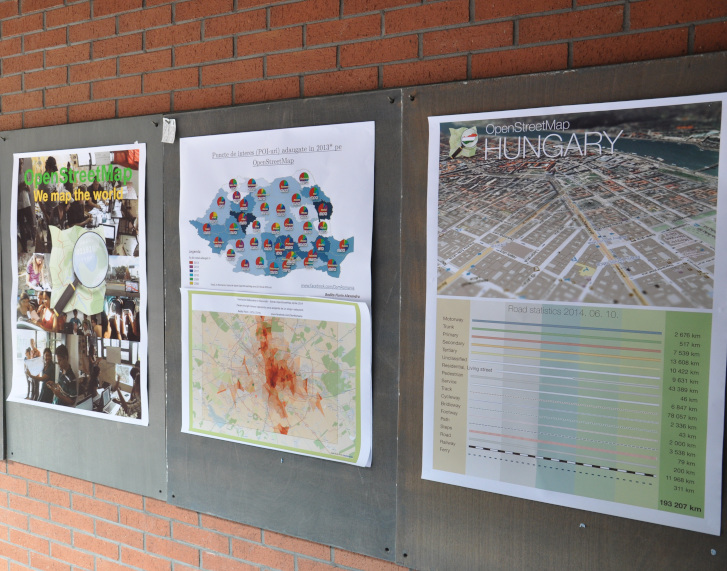
\includegraphics[width=0.9\linewidth]{images-print/posters-sotm-eu-2014.jpg}

            \qrcode[height=18mm,padding]{geo:49.41722,8.67550}%
          \end{center}
        \end{minipage}
      \end{minipage}
      \vspace{0.4\multicolsep}
      \tabularnewline
      \programHRule{2}
    \end{tabular}
  \end{center}
\end{landscape}
\renewcommand{\arraystretch}{1.0}
\normalsize

\newpage
\small
\renewcommand{\arraystretch}{1.4}
%\section*{Monday Schedule}
\label{monday}
\pagestyle{monday-table}
\setPageBackground
\noindent\begin{landscape}
  \begin{center}
    \noindent\begin{tabular}{Z{0.75cm}Z{2.38cm}|Z{2.38cm}|Z{2.38cm}|Z{2.38cm}|}
      \cellcolor{commongray}
      & \multicolumn{1}{c}{\cellcolor{GHS} Großer Hörsaal}
      & \multicolumn{1}{c}{\cellcolor{HSO} Hörsaal Ost}
      & \multicolumn{1}{c}{\cellcolor{KHS} Kleiner Hörsaal~\noVideo}
      & \multicolumn{1}{c}{\cellcolor{Mathematikon C} Mathematikon C~\noVideo}
      \tabularnewline
      \cellcolor{commongray}
      09:30
      \talk{Qwant Maps: Geocode the World with OSM Data}{Guillaume et\,al.}
      \talk{OSM2World: 3D OSM in Your Browser}{Tobias Knerr}
      \longTalk{2}{The Next Generation of Mappers: Learning from YouthMappers}{Jessica Bergmann}
      \longTalk{2}{\emph{Workshop}\linebreak OpenStreetMap and Wikidata: Awesome Together}{Eugene Alvin Villar}
      \tabularnewline
      \programCRule{2-3}
      \cellcolor{commongray}
      10:00
      \talk{Routing for \mbox{Humans}}{Sebastian Ritterbusch}
      \talk{OpenDatathon Activities in Japan}{Shinji Enoki}
      &
      &
      \tabularnewline
      \programHRule{5}
      \cellcolor{commongray}
      10:30
      \talk{Mapping Mobility in Stockport}{Sam Milson}
      \talk{Lightning Talks IV}{}
      \talk{OpenStreetMap in Croatia}{Hrvoje Bogner}
      &
      \tabularnewline
      \rowcolor{commongray}
      11:00
      & \multicolumn{4}{c}{%
      \parbox[c]{24pt}{%
        
\includegraphics[height=10pt]{cafe}%
      }
      Break}
    \end{tabular}

    \noindent\begin{tabular}{Z{0.75cm}Z{2.38cm}|Z{2.38cm}|Z{2.38cm}|Z{2.38cm}|}
      \cellcolor{commongray}
      & \multicolumn{1}{c}{\cellcolor{GHS} Großer Hörsaal}
      & \multicolumn{1}{c}{\cellcolor{HSO} Hörsaal Ost}
      & \multicolumn{1}{c}{\cellcolor{KHS} Kleiner Hörsaal~\noVideo}
      & \multicolumn{1}{c}{\cellcolor{Mathematikon C} Mathematikon C~\noVideo}
      \tabularnewline
      \cellcolor{commongray}
      11:30
      \longTalk{2}{Caretography~-- Mapping Difficult Issues with OpenStreetMap during Difficult Times}{David Garcia, Martin Dittus}
      \talk{Integrating and Validating Open Data in OSM Using Street Pictures}{Andrien Pavie}
      \longTalk{2}{New processes to Agree on Tagging Suggestions and Their Interaction with the Editing Software Available on osm.org}{Roland Olbricht}
      \longTalk{2}{\emph{Workshop}\linebreak Custom Presets Creation Using JOSM}{Harry Mahardhika Machmud}
      \tabularnewline
      \programCRule{3-3}
      \cellcolor{commongray}
      12:00
      &
      \talk{Introduce OpenPlaceReviews and Connect to OSM}{Victor Shcherb}
      &
      &
      \tabularnewline
      \programHRule{5}
      \cellcolor{commongray}
      12:30
      \talk{Access to\linebreak Prosperity: Quantifying Infrastructure Impact with OSM}{Davey Lovin}
      \talk{Lightning Talks VII}{}
      &
      &
      \tabularnewline
      \rowcolor{commongray}
      13:00
      & \multicolumn{4}{c}{%
        \parbox[c]{24pt}{%
          
\includegraphics[height=10pt]{restaurant}%
        }
      Lunch}
    \end{tabular}

    \noindent\begin{tabular}{Z{0.75cm}Z{2.38cm}|Z{2.38cm}|Z{2.38cm}|Z{2.38cm}|}
      \cellcolor{commongray}
      & \multicolumn{1}{c}{\cellcolor{GHS} Großer Hörsaal}
      & \multicolumn{1}{c}{\cellcolor{HSO} Hörsaal Ost}
      & \multicolumn{1}{c}{\cellcolor{KHS} Kleiner Hörsaal~\noVideo}
      & \multicolumn{1}{c}{\cellcolor{Mathematikon C} Mathematikon C~\noVideo}
      \tabularnewline
      \cellcolor{commongray}
      14:00
      \talk{Pedestrian Routing in Complex Areas: the Case of Paris Railway Stations}{Antoine Riche}
      \talk{Norway: Successful Deployment of OSM in Public Transport}{Johan Wiklund}
      \talk{Participatory Mapping for Open Counties}{Zacharia Muindi}
      \longTalk{2}{\emph{Workshop}\linebreak ImproveOSM~-- MissingRoads Workshop}{Beata Tautan-Jancso, Dumitru Laura}
      \tabularnewline
      \programCRule{2-4}
      \cellcolor{commongray}
      14:30
      \talk{Automatically\linebreak Annotate a Pedestrian Route with OSM Landmarks}{Frédéric Rodrigo}
      \talk{Public Transport Navigation Using OSM by OsmAnd}{Victor Shcherb, Eugene Kizevich}
      &
      &
      \tabularnewline
      \programHRule{5}
      \cellcolor{commongray}
      15:00
      \talk{From Car Routing to Train Routing~\noVideo}{Denis Cheynet}
      \talk{OSM Vector Tiles in Custom Coordinate Systems}{Jiri Komarek}
      \talk{State of the Map Bangladesh: Transforming a Resilient Community by Institutionalising~\diamondSymbol}{Tasauf A Baki Billah}
      &
      \tabularnewline
      \rowcolor{commongray}
      15:30
      & \multicolumn{4}{c}{%
      \parbox[c]{24pt}{%
        
\includegraphics[height=10pt]{cafe}%
      }
      Break}
      \tabularnewline
      \cellcolor{commongray}
      16:00
      \talk{Closing}{}
      &
      &
      &
      \tabularnewline
      \programHRule{5}
    \end{tabular}
  \end{center}
  \renewcommand{\arraystretch}{1.0}

  \newpage
  \pagestyle{cropmarksstyle}
  \sponsorBoxLandscape{%
    images-print/osmf-banner.png%
  }{%
    40mm
  }{%
    4
  }{%
    The OpenStreetMap Foundation is the 
    international non-profit organisation
    supporting, but not controlling,
    OpenStreetMap. We are dedicated to
    encouraging the growth, development and
    distribution of free geospatial data and to
    providing geospatial data for anyone to use
    and share.
    
    We need you as member. Members are vital
    to the OpenStreetMap Foundation---to voice ideas
    and shape the direction of the Foundation,
    and support efforts of working groups. We
    welcome all who support our goals to join us!
    
    Find out more and join at osmfoundation.org
    or join our sessions:
    \begin{itemize}
      \RaggedRight
      \setlength{\itemsep}{-3pt} % Aufzählungspunktabstand auf 0
      \item Saturday 14:00, Großer Hörsaal: ODbL licence compatiblity
      \item Saturday 15:00, Großer Hörsaal: Past and Future of the OSMF Membership Working Group
      \item Saturday 16:30, Hörsaal West: Board and working groups meeting
      \item Sunday 16:30, Kleiner Hörsaal: Updating our attribution guidelines
      \item Sunday 17:00, Kleiner Hörsaal: Local chapter congress
    \end{itemize}
    \justifying
  }%


  \setlength{\fboxsep}{4.5pt}%
  \vspace{0.5\baselineskip}%
  \noindent%
  \fcolorbox{gray}{white}{%
    \parbox{\fboxwidth}{%
      \parbox{0.82\fboxwidth}{%
        \noindent Video recording and streaming is provided
        by the volunteers of CCC Video Operation Centre.
        The videos will be published at https://media.ccc.de/ under
        a free and open licence.
      }%
      \hfill%
      \parbox{0.15\fboxwidth}{%
        \begin{center}
          
\includegraphics[width=12mm]{images-print/voc.pdf}%
        \end{center}
      }%
    }%
  }
  \setlength{\fboxsep}{3pt}

\end{landscape}

\newpage

\newpage
\section*{Saturday Sessions Descriptions}\label{saturday-descriptions}
\renewcommand{\conferenceDay}{\saturday}
\setPageBackground
% time: Saturday 09:30
% URL: https://pretalx.com/sotm2019/talk/HFET3E/

%
\newSmallTimeslot{09:30}
\abstractGHS{%
}{%
  Opening%
}{%
}{%
}


%%%%%%%%%%%%%%%%%%%%%%%%%%%%%%%%%%%%%%%%%%%

% time: Saturday 10:00
% URL: https://pretalx.com/sotm2019/talk/TWARHC/

%
\newSmallTimeslot{10:00}
\abstractGHS{%
  Dietmar Seifert, Christian Förster%
}{%
  \emph{Keynote} Open up! Why digital mobility needs participation%
}{%
}{%
  Baden-Württemberg’s Ministry of Transport aims at developing regional mobility data towards an
  open and interoperable framework for new mobility solutions~-- as part of a sustainable traffic
  system, realising efficiency, climate protection and living quality. On the way there, fair
  chances for innovation are key: Not only for better results but also for the involvement of most
  different societal actors. Cross-thinking and open innovation are cornerstones in such a process.%
}


%%%%%%%%%%%%%%%%%%%%%%%%%%%%%%%%%%%%%%%%%%%

% time: Saturday 10:30
% URL: https://pretalx.com/sotm2019/talk/VC8ESD/

%
\newSmallTimeslot{10:30}
\abstractGHS{%
  Karen M. Sandler%
}{%
  \emph{Keynote}%
}{%
}{%
  Karen M. Sandler is the executive director of the Software Freedom Conservancy, which is the
  nonprofit home of dozens of free and open source software projects including Git, Etherpad, QEMU,
  Selenium and Inkscape (to name but a few). She is known as a cyborg lawyer for her advocacy for free
  software as a life-or-death issue, particularly in relation to the software on medical devices.

%  Prior to joining the Conservancy, she was the executive director of the GNOME Foundation. Before
%  that, she was the general counsel of the Software Freedom Law Center.
  She co-organizes
  Outreachy, the award-winning outreach programme for people who are subject to systemic bias and
  underrepresented in tech.
  Karen is an adjunct Lecturer-In-Law at Columbia Law School and a
  Visiting Scholar at UC Santa Cruz. She is the recipient of the Free Software Foundation's 2017
  Award for the Advancement of Free Software as well as an O'Reilly Open Source Award.
}


%%%%%%%%%%%%%%%%%%%%%%%%%%%%%%%%%%%%%%%%%%%

% time: Saturday 11:30
% URL: https://pretalx.com/sotm2019/talk/VZVFMS/

%
\newSmallTimeslot{11:30}
\abstractGHS{%
  Astrid Emde%
}{%
  Get to know OSGeo and how OSGeo is connected to OpenStreetMap%
}{%
  Open Source Software and Open Education making use of OSM data
}{%
  OSGeo is all about open source software, open data and open education. Learn about OSGeo and what
  builds up this great organization and find out how OpenStreetMap is used by OSGeo projects, how
  OSM can use OSGeo projects and how the two OSGeo and OSM are connected.%
}


%%%%%%%%%%%%%%%%%%%%%%%%%%%%%%%%%%%%%%%%%%%

% time: Saturday 11:30
% URL: https://pretalx.com/sotm2019/talk/7ZXRXB/

%

\abstractHSO{%
  Olivier Courtin \speakerAffiliation{DataPink}
}{%
  Data Quality and Feature Extraction at scale with RoboSat.pink%
}{%
}{%
  How to use plain open data and imagery to train an accurate deep learning model, able to detect
  inconsistencies in an OSM dataset, to spot it and to extract features.
  And make it work at scale, with open source solution named RoboSat.pink.%
}


%%%%%%%%%%%%%%%%%%%%%%%%%%%%%%%%%%%%%%%%%%%

% time: Saturday 11:30
% URL: https://pretalx.com/sotm2019/talk/NPYVSP/

%

\abstractHSW{%
  Thomas Skowron, Frederik Ramm%
}{%
  Introduction to OSM: How it's made and how it's used%
}{%
}{%
  This session provides an entertaining yet informative introduction into everything you need to
  know about OpenStreetMap.%
}


\newpage

%%%%%%%%%%%%%%%%%%%%%%%%%%%%%%%%%%%%%%%%%%%

% time: Saturday 11:30
% URL: https://pretalx.com/sotm2019/talk/Z9VBKM/


\abstractKHS{%
  Polyglot%
}{%
  Mapping public transport and cycling itineraries using JOSM's PT\_Assistant plugin~\noVideo %
}{%
}{%
  The PT\_Assistant plugin has been developed over the past 3 summers as a Google Summer of Code project and will
  probably see further development this summer. During this workshop, learn how
  PT\_Assistant can map itineraries for public transport, cycling and hiking.
  Bring a computer with Java installed on it to take part interactively.
}

%%%%%%%%%%%%%%%%%%%%%%%%%%%%%%%%%%%%%%%%%%%

% time: Saturday 12:00
% URL: https://pretalx.com/sotm2019/talk/3WQKAX/

%
\newSmallTimeslot{12:00}
\abstractGHS{%
  Christopher Klaiber \speakerAffiliation{Facebook}, Kevin Ventullo \speakerAffiliation{Facebook}%
}{%
  ``Keepin' it fresh (and good)!''%
}{%
  Continuous Ingestion of OSM Data at Facebook%
}{%
  Building forward from our work on Mobius Logical Changesets (presented last year at SotM US 2018),
  we have created an automated ingestion framework for OSM data that allows us to selectively update
  parts of the map instead of doing a full snapshot change.%
}


%%%%%%%%%%%%%%%%%%%%%%%%%%%%%%%%%%%%%%%%%%%

% time: Saturday 12:00
% URL: https://pretalx.com/sotm2019/talk/KAPNKV/

%

\abstractHSO{%
  Christopher Beddow \speakerAffiliation{Mapillary}, Edoardo Neerhut \speakerAffiliation{Mapillary}%
}{%
  Human Mapping with Machine Data%
}{%
}{%
  How useful are map features automatically extracted from street-level images? Can they be trusted?
  These are some of the questions we tried to answer through community campaigns and student-led
  research in 2019. We will share some of these lessons and elicit a broader discussion on the
  methods that can be used to turn automatically extracted features into useful OpenStreetMap data.%
}


%%%%%%%%%%%%%%%%%%%%%%%%%%%%%%%%%%%%%%%%%%%

% time: Saturday 12:30
% URL: https://pretalx.com/sotm2019/talk/PAG8CN/

%
\newSmallTimeslot{12:30}
\abstractGHS{%
  Jinal Foflia \speakerAffiliation{Grab}%
}{%
  Driving South East Asia Forward with OpenStreetMap%
}{%
}{%
  It’s been more than a year since we at Grab incorporated OpenStreetMap into our ecosystem and we
  have come a long way since then. This talk will focus on our learning journey, our tools, the
  challenges and our experiences working in the South East Asia region and the vibrant OpenStreetMap
  communities here.%
}


%%%%%%%%%%%%%%%%%%%%%%%%%%%%%%%%%%%%%%%%%%%

% time: Saturday 12:30
% URL: https://pretalx.com/sotm2019/talk/DPGWFB/

%

\abstractHSO{%
  Felix Delattre \speakerAffiliation{HOT}, Surabhi Singh \speakerAffiliation{Microsoft/HOT}%
}{%
  Assisted Intelligence~-- How we map with the support of new technologies%
}{%
}{%
  Deep learning methods for feature extraction using computer vision are giving concrete results.
  This talk provides an overview of feature detection from satellite imagery and how machine
  learning can provide a seamless mapping experience for mappers, allowing them to utilize their
  knowledge to enrich maps further.%
}

\newpage

%%%%%%%%%%%%%%%%%%%%%%%%%%%%%%%%%%%%%%%%%%%

% time: Saturday 14:30
% URL: https://pretalx.com/sotm2019/talk/UN33XK/

%
\newSmallTimeslot{14:30}
\abstractGHS{%
  Kathleen Lu \speakerAffiliation{LWG}%
}{%
  ODbL license compatibility%
}{%
}{%
  Have you ever wondered if a certain dataset can be used for OSM? What does it mean for a license to be
  ``compatible'' with OSM and ODbL? This talk will give pointers on where to look for information,
  common compatibility issues, and best practices for presenting a license to the Licensing Working Group (LWG) for help review.%
}



%%%%%%%%%%%%%%%%%%%%%%%%%%%%%%%%%%%%%%%%%%%

% time: Saturday 14:30
% URL: https://pretalx.com/sotm2019/talk/FLPYCN/

%

\abstractHSO{%
}{%
  Lightning Talks I%
}{%
}{%
  %TODO adapt space
  \vspace{-1.5em}
  \begin{itemize}
    \RaggedRight
    \setlength{\itemsep}{-3pt} % Aufzählungspunktabstand auf 0
    \lightningTalk{Uses of native language in OSM}{S M Sawan Shariar \speakerAffiliation{YouthMappers Dhaka College}}
    \lightningTalk{SolidaryCityMap}{OpenDEM}
    \lightningTalk{OpenLitterMap~-- open data on plastic pollution with blockchain rewards (Littercoin)}{Seán Lynch \speakerAffiliation{OpenLitterMap}}
    \lightningTalk{Map2endFGM}{Janet Chapman \speakerAffiliation{Crowd2Map Tanzania}}
  \end{itemize}%
  \justifying
}

%%%%%%%%%%%%%%%%%%%%%%%%%%%%%%%%%%%%%%%%%%%

% time: Saturday 14:30
% URL: https://pretalx.com/sotm2019/talk/N9RCV8/


\abstractHSW{%
  Roland Olbricht%
}{%
  Share Edits and Insights with the Overpass Tools%
}{%
}{%
  Not every data item in OpenStreetMap can have an immediate impact on the rendered map. But you can
  make every data item visible on a map and share the links or share the data, no matter how much
  the item is special interest. This is the purpose of Overpass API and Overpass Turbo.%
}

\newpage

%%%%%%%%%%%%%%%%%%%%%%%%%%%%%%%%%%%%%%%%%%%
% time: Saturday 14:30
% URL: https://pretalx.com/sotm2019/talk/JJUFQT/


\abstractKHS{%
  Manfred Reiter%
}{%
  How to contribute to weeklyOSM via the CMS~-- OSMBC~\noVideo%
}{%
  The OSM community should know about it~\dots%
}{%
  OSMBC is the Content Management System to produce weeklyOSM in recently nine languages.%
}

%%%%%%%%%%%%%%%%%%%%%%%%%%%%%%%%%%%%%%%%%%%

% time: Saturday 15:00
% URL: https://pretalx.com/sotm2019/talk/R3BAWM/

%
\newSmallTimeslot{15:00}
\abstractGHS{%
  Hanna Krüger%
}{%
  Communication and Knowledge Transfer in OpenStreetMap%
}{%
}{%
  The OpenStreetMap project uses many different technologies and channels for communication and documentation. This talk is an overview of various communication platforms and their relevance and reach at local and international level. In addition, the advantages and disadvantages of the current strategy for communication and knowledge transfer will be discussed.
}


%%%%%%%%%%%%%%%%%%%%%%%%%%%%%%%%%%%%%%%%%%%

% time: Saturday 15:00
% URL: https://pretalx.com/sotm2019/talk/VAADJ9/

%

\abstractHSO{%
  Thomas Sontag, Andreas Dirks, Hannes Geißelmann, Adrien Pavie%
}{%
  OsmInEdit: a simple indoor editor%
}{%
}{%
  The Indoor Map Creator is an easy-to-use open-source map editor for OSM indoor data. It is
  web-based with an intuitive user interface to make mapping indoors accessible and easy for
  everyone. Check it out and enjoy mapping buildings!%
}

\newpage

%%%%%%%%%%%%%%%%%%%%%%%%%%%%%%%%%%%%%%%%%%%

% time: Saturday 15:30
% URL: https://pretalx.com/sotm2019/talk/FAGNLA/

%
\newSmallTimeslot{15:30}
\abstractGHS{%
  Michael Spreng%
}{%
  Past and Future of the OSMF Membership Working Group%
}{%
}{%
  What is an OSMF working group? What does the membership working group in particular do? and how
  can you improve the experience of an OSMF membership?%
}


%%%%%%%%%%%%%%%%%%%%%%%%%%%%%%%%%%%%%%%%%%%

% time: Saturday 15:30
% URL: https://pretalx.com/sotm2019/talk/39SBT8/
%

\enlargethispage{1\baselineskip}

\abstractHSO{%
  Sajjad Anwar%
}{%
  Observe~-- offline, cross-platform field mapping tool for OpenStreetMap%
}{%
}{%
  Over the last few months, we’ve been building an offline first field mapping tool for the
  OSM ecosystem called Observe. Observe makes field surveying, and verification easy for
  mappers, and works on iOS and Android. My talk will cover how Observe integrates with mapping
  workflows and helps improve OSM data from the field. I'll also touch upon fundamentals of building
  Observe and our assumptions on field mapping.%
}


%%%%%%%%%%%%%%%%%%%%%%%%%%%%%%%%%%%%%%%%%%%

% time: Saturday 16:30
% URL: https://pretalx.com/sotm2019/talk/799WZF/

%
\newSmallTimeslot{16:30}
\abstractGHS{%
  Yantisa Akhadi \speakerAffiliation{HOT}%
}{%
  OSM Data: From Digital to Physical Design%
}{%
}{%
  Exploring the visualization of OSM data outside its digital form and how it can be applied to
  everyday objects from book covers to wallpaper. This talk will discuss how to elevate OSM data
  beyond maps, exploring its potential in data-as-decor in both public and private space. The talk
  will describe the tools and workflow used to create these products as well as its strengths and
  weaknesses.%
}

\newpage

%%%%%%%%%%%%%%%%%%%%%%%%%%%%%%%%%%%%%%%%%%%
% time: Saturday 16:30
% URL: https://pretalx.com/sotm2019/talk/BBRMPZ/

%

\abstractHSO{%
}{%
  Lightning Talks II%
}{%
}{%
  %TODO adapt space
  \vspace{-1em}
  \begin{itemize}
    \RaggedRight
    \setlength{\itemsep}{-3pt} % Aufzählungspunktabstand auf 0
    \lightningTalk{OpenStreetMap intrinsic quality assessment using ``Is OSM up-to-date?'' web application}{Marco Minghini, Francesco Frassinelli}
    \lightningTalk{Deriviste~-- Click and Go Photo Mapping}{Christopher Beddow \speakerAffiliation{Mapillary}}
    \lightningTalk{Fifty states in 12 years and five minutes}{Minh Nguyễn}
    \lightningTalk{``MAPAbabae'': Using OSM as a Tool for Mapping with Women and For Women}{Andi Tabinas, Arnalie Vicario}
    \lightningTalk{Send me a postcard}{Ilya Zverv}
  \end{itemize}%
  \justifying
}


%%%%%%%%%%%%%%%%%%%%%%%%%%%%%%%%%%%%%%%%%%%

% time: Saturday 16:30
% URL: https://pretalx.com/sotm2019/talk/9MR9QK/

%

\abstractHSW{%
  Joost Schouppe \speakerAffiliation{OSMF}%
}{%
  OSMF Board + Working Groups meeting%
}{%
}{%
  Get to know the Board and the Working Groups. Together, we run the OSMF. Let's use the SotM to
  have a real face-to-face meeting. The public is invited to join the conversation too.%
}

%%%%%%%%%%%%%%%%%%%%%%%%%%%%%%%%%%%%%%%%%%%

% time: Saturday 16:30
% URL: https://pretalx.com/sotm2019/talk/J7D7UU/


\abstractKHS{%
  Manfred Reiter%
}{%
  uMap for newbies~\noVideo%
}{%
}{%
  We create an individualized map based on OSM using uMap.%
}

%%%%%%%%%%%%%%%%%%%%%%%%%%%%%%%%%%%%%%%%%%%

% time: Saturday 17:00
% URL: https://pretalx.com/sotm2019/talk/SBDEU8/

%
\newSmallTimeslot{17:00}
\abstractGHS{%
  Florimond Berthoux, Lucas Verney%
}{%
  CyclOSM, a bicycle oriented render for every cyclist%
}{%
}{%
  CyclOSM is a new cycling render. It is free and aims at rendering new bicycle-specific features,
  in order to take into account the diversity of cycling practices.%
}


%%%%%%%%%%%%%%%%%%%%%%%%%%%%%%%%%%%%%%%%%%%

% time: Saturday 17:00
% URL: https://pretalx.com/sotm2019/talk/9TMRYN/

%

\abstractHSO{%
  Robert Kaiser \speakerAffiliation{Mozilla}%
}{%
  VR Map: Using OSM Data In a WebVR Environment%
}{%
  Simple GeoData Visualization with A-Frame
}{%
  Can you actually walk through or fly over a 3D scene of live OSM data using a VR headset?~-- and if
  so, can this be done in a way that easily transforms to a view on a normal computer (or mobile)
  screen?
  The answers are ``Yes'' and ``Yes'', and this talk will show how this can be done with relatively
  simple code, and all inside a web browser!%
}


%%%%%%%%%%%%%%%%%%%%%%%%%%%%%%%%%%%%%%%%%%%

% time: Saturday 17:30
% URL: https://pretalx.com/sotm2019/talk/JNXE9Q/

%
\newSmallTimeslot{17:30}
\abstractGHS{%
  Astrid Emde \speakerAffiliation{OSGeo}%
}{%
  How to Use OpenStreetMap Data with the Desktop GIS QGIS%
}{%
  Get to Know the Great Combination of OSM Data and QGIS%
}{%
  The desktop GIS QGIS offers many ways to work with OSM data. This presentation will give
  an overview on how you can use OSM data with QGIS.%
}


%%%%%%%%%%%%%%%%%%%%%%%%%%%%%%%%%%%%%%%%%%%

% time: Saturday 17:30
% URL: https://pretalx.com/sotm2019/talk/DETEML/

%

\abstractHSO{%
  Nick Whitelegg \speakerAffiliation{Solent University}%
}{%
  Hikar~-- OSM Augmented Reality for Walkers across Europe%
}{%
}{%
  Hikar is an OSM-based augmented reality navigation app for walkers and hikers, showing OSM ways
  overlaid on the camera feed of the device and, in the latest version, virtual signposts pointing
  the way to nearby points of interest. This technical talk will introduce Hikar, detail the many
  new developments since it was last presented at SotM Birmingham 2013, and describe how it works in
  technical detail.%
}

\enlargethispage{2\baselineskip}

%%%%%%%%%%%%%%%%%%%%%%%%%%%%%%%%%%%%%%%%%%%

\newSmallTimeslot{19:00}
\abstractOther{%
}{%
  Social Event%
}{%
}{%
  See page~\pageref{social-event} for details about the social event.
}{%
  Hebelhalle%
}

\newpage
\section*{Sunday Sessions Descriptions}\label{sunday-descriptions}
\renewcommand{\conferenceDay}{\sunday}
\setPageBackground
\newSmallTimeslot{09:00}
\abstractAcademic{%
  A. Yair Grinberger \speakerAffiliation{Heidelberg University},
  Marco Minghini \speakerAffiliation{European Commission, Joint Research Centre},
  Levente Juhász \speakerAffiliation{Florida International University},
  Peter Mooney \speakerAffiliation{Maynooth University},
  Godwin Yeboah \speakerAffiliation{University of Warwick} 
}{%
  Bridging the Map?%
}{%
  Exploring Interactions between the Academic and Mapping Communities in OpenStreetMap
}{%
  This talk presents an initial inquiry into the relations between the academic and mapping
  communities in OpenStreetMap, based on a review of recent publications, interviews of colleagues,
  and self-reflection of the authors. By this, we aim to understand how and when research-community
  interactions come to be, what is their nature, and how these can be improved and made more
  productive for both sides.
}


% time: Sunday 09:30
% URL: https://pretalx.com/sotm2019/talk/P8AG7K/

\newSmallTimeslot{09:30}
\abstractGHS{%
  Peter Karich \speakerAffiliation{GraphHopper GmbH}%
}{%
  Flexible Routing with GraphHopper%
}{%
}{%
  In this talk we give an overview on how to use GraphHopper to provide more flexible routing
  (based on weather information, road class, road width,\dots) and how this could be also used for
  visualization purposes or data analysis.%
}

%%%%%%%%%%%%%%%%%%%%%%%%%%%%%%%%%%%%%%%%%%%

% time: Sunday 09:30
% URL: https://pretalx.com/sotm2019/talk/GQ3AAF/


\abstractHSO{%
  Nicolas Chavent, Séverin Menard \speakerAffiliation{LLG/ProjetEOF}%
}{%
  "`Mapathon, mapathon, mapathon!"'%
}{%
}{%
  Who benefits from mapathons? Between (over)communication and (over)attribution, critical
  feedback on the inflation of a form of action oversold in the field of humanitarian action and
  development aid. Do they really benefit OSM?%
}

\abstractAcademic{%
  Dipto Sarkar \speakerAffiliation{National University of Singapore}, So Hoi Kay \speakerAffiliation{ibid.}
}{%
  OpenStreetMap as a Space~\noVideo
}{%
}{%
  Can OSM be used in classroom teaching as a definitive instance of a geographic space? We provide
  instances of how OSM as space may be of interest to researchers and for students of geography
  alike. Concepts of human geography manifested in OSM can be used to understand how digital
  geographies and offline activities are intrinsically interwoven with and influenced by each other.
  Thus, introduction to digital geography in classrooms can be through concepts in human geography.
}

%%%%%%%%%%%%%%%%%%%%%%%%%%%%%%%%%%%%%%%%%%%

% time: Sunday 09:30
% URL: https://pretalx.com/sotm2019/talk/PRHPXV/


\abstractKHS{%
}{%
  Scholar Lightning Talks~\noVideo%
}{%
}{%
  %TODO adapt space
  \vspace{-1em}
  \begin{itemize}
    \RaggedRight
    \setlength{\itemsep}{-3pt} % Aufzählungspunktabstand auf 0
    \lightningTalk{Mapping Advocacy: Breastfeeding stations in the Philippines}{Jen Alconis Ayco}
    \lightningTalk{Open data for disaster governance in Nepal}{Pradip Khatiwada \speakerAffiliation{Youth Innovation Lab}}
    \lightningTalk{MapLesotho}{Tshedy Letsie}
    \lightningTalk{State of the Map~-- India}{Naveen Francis}
    \lightningTalk{OSM for Gambia (mapping the whole Gambia)}{Jariatou Jallow \speakerAffiliation{Connected YouthMappers}}
    \lightningTalk{HOT and OSM in Tanzania, the ups and downs of crowdsourced mapping}{Emmor Nile}
    \lightningTalk{Community cartographers}{Fernando Castro T \speakerAffiliation{Fundación OpenStreetMap Colombia}}
    \lightningTalk{Using OpenStreetMap building footprints data for population distribution model: a case study in Cavite, Philippines}{Dinnah Feye H. Andal}
    \lightningTalk{Public transport in OSM}{Porfirio Carrasco}
    \lightningTalk{Rendering order in openstreetmap-carto}{Matthijs Melissen}
  \end{itemize}%
  \justifying
}

%%%%%%%%%%%%%%%%%%%%%%%%%%%%%%%%%%%%%%%%%%%

% time: Sunday 10:00
% URL: https://pretalx.com/sotm2019/talk/TVSA9F/

\newSmallTimeslot{10:00}
\abstractGHS{%
  Kevin Bullock \speakerAffiliation{Maxar}%
}{%
  Imagery Solutions in OpenStreetMap%
}{%
}{%
  Satellite imagery has materially enhanced OpenStreetMap and improved editing and validation. In
  this talk we present recent enhancements we have made to get even more information from
  satellite imagery.%
}

%%%%%%%%%%%%%%%%%%%%%%%%%%%%%%%%%%%%%%%%%%%

% time: Sunday 10:00
% URL: https://pretalx.com/sotm2019/talk/VWBV88/


\abstractHSO{%
  Séverin Menard, Nicolas Chavent \speakerAffiliation{LLG/ProjetEOF}%
}{%
  OSMF local chapters in countries of the Global South
}{%
  What can we learn from OSM associations dynamics in French-speaking southern countries of Africa and the Caribbean?%
}{%
  This talk will share lessons that OSM and OSMF members can learn about the multi-year collective
  dynamics around OpenStreetMap which unfold in French-speaking southern countries of Africa and the
  Caribbean with the view to identifying paths for local OSM grassroots groups' evolution toward becoming
  formal OSMF Local Chapters.%
}

\abstractAcademic{%
  Toshikazu Seto \speakerAffiliation{University of Tokyo}, Hiroshi Kanasugi,
  \speakerAffiliation{ibid.}, Yuichiro Nishimura \speakerAffiliation{Nara Women's University}
}{%
  Analysis of OSM data through OSM Notes user posting
}{%
}{%
  In this research, the OSM Notes feature is mainly viewed as data that can be examined speedily from global OSM data in terms of the content of the notes posted and the location of users.
}

\newpage

%%%%%%%%%%%%%%%%%%%%%%%%%%%%%%%%%%%%%%%%%%%

% time: Sunday 10:30
% URL: https://pretalx.com/sotm2019/talk/EGMAVR/

\newSmallTimeslot{10:30}
\abstractGHS{%
}{%
  Lightning Talks III%
}{%
}{%
  %TODO adapt space
  \vspace{-2em}
  \begin{itemize}
    \RaggedRight
    \setlength{\itemsep}{-3pt}
    \lightningTalk{Human in the Loop: Verifying Machine-Generated Data for Better Maps}{Katrin Humal \speakerAffiliation{Mapillary}}
    \lightningTalk{Share the word}{Ilya Zverev \speakerAffiliation{Juno Lab}}
    \lightningTalk{Enhancing OSM with missing roads}{Beata Tautan-Jancso \speakerAffiliation{Telenav}}
    \lightningTalk{Community-led mapping helping in policy changes}{Sibabrata Choudhury \speakerAffiliation{Envision}}
    \lightningTalk{How to create a data annotation process used for navigation}{Alina Negreanu}
  \end{itemize}%
  \justifying
}

%%%%%%%%%%%%%%%%%%%%%%%%%%%%%%%%%%%%%%%%%%%

% time: Sunday 10:30
% URL: https://pretalx.com/sotm2019/talk/7Q97AH/


\abstractHSO{%
  Ramya Ragupathy \speakerAffiliation{HOT}, Wille Marcel Lima Malheiro, Felix Delattre \speakerAffiliation{HOT}%
}{%
  Tales from the Tasking Manager%
}{%
}{%
  The Tasking Manager is OpenStreetMap’s most used software tool to organize mapathons, community
  mapping initiatives, and professional mapping teams. Over the last year it has been developed
  further significantly. This talk will give an update on the newest developments and the emerging
  community around the application.%
}

\abstractAcademic{%
  Peter Mooney \speakerAffiliation{Maynooth University}
}{%
  A novel application of models of species abundance to better understand OpenStreetMap Community structure and interactions
}{%
}{%
  The OSM community is a global community crossing cultures, languages, and geographical boundaries. Researchers have been working to develop automated approaches to understanding the composition of this community through their contributions to the OSM database. In this talk we propose a new and novel application of theories and models of species abundance from ecological science to understand contributor community structure and distributions in OSM.
}


%%%%%%%%%%%%%%%%%%%%%%%%%%%%%%%%%%%%%%%%%%%

% time: Sunday 11:30
% URL: https://pretalx.com/sotm2019/talk/YFUEBH/

\newSmallTimeslot{11:30}
\abstractGHS{%
  Paul Norman%
}{%
  Overview of map serving architectures%
}{%
}{%
  Serving maps is one of the most common uses of OpenStreetMap data. This talk goes over the
  component-level architecture for common and uncommon ways to serve maps.%
}

%%%%%%%%%%%%%%%%%%%%%%%%%%%%%%%%%%%%%%%%%%%

% time: Sunday 11:30
% URL: https://pretalx.com/sotm2019/talk/YENWFX/


\abstractHSO{%
  Alison Moon \speakerAffiliation{thinkWhere}%
}{%
  ``Our Falkirk''
}{%
  Mitigating the Impacts of Poverty using OSM Data Themes%
}{%
  Services that provide money advice, access to food provision, digital access, and community support
  are key to supporting people facing poverty.  ``Our Falkirk'' is a simple mapping platform for
  service discovery that allows enriched OSM data to be easily described, mapped and shared through
  the concept of data ‘themes’.%
}


\abstractAcademic{%
  Rui Zhang \speakerAffiliation{IBM Research},
  Marcus Freitag \speakerAffiliation{ibid.},
  Conrad Albrecht \speakerAffiliation{ibid.},
  Siyuan Lu \speakerAffiliation{ibid.},
  Wei Zhang \speakerAffiliation{ibid.}
}{%
  Towards Scalable Geospatial Remote Sensing for Efficient OSM Labeling
}{%
}{%
  The time OSM mappers invest in labeling the world is valuable. We present how methods from remote
  sensing, big data distributed computing, and artificial intelligence can be combined to support
  human analysis of geo-spatial data.
}


%%%%%%%%%%%%%%%%%%%%%%%%%%%%%%%%%%%%%%%%%%%

% time: Sunday 11:30
% URL: https://pretalx.com/sotm2019/talk/NCSSPK/


\abstractKHS{%
  Nicolas Chavent \speakerAffiliation{LLG/ProjetEOF}, Séverin Ménard
}{%
  Bilingual Breakout Session~\noVideo%
}{%
}{%
  This session will present the rise of active, self-standing grassroots communities in Haiti,
  Western and Central Africa since 2010 resulting from a unique set of continued support actions
  replicable in other territories, by an ensemble of speakers from (at least) France, Burkina Faso,
  Senegal and Togo.

  The following people will speak during this session:
  %TODO adapt space
  %\vspace{-2em}
  \begin{itemize}
    \RaggedRight
    \setlength{\itemsep}{-3pt}
    \item Nicolas Chavent (France)
    \item Séverin Ménard (France)
    \item Amadou Ndong (Senegal)
    \item Aimée Sama (Togo)
    \item Innocent Dibloni (Burkina Faso)
    \item Saliou Abdou (Benin)
    \item Racky Ly (Ivory Coast)
  \end{itemize}%
  \justifying
}

%%%%%%%%%%%%%%%%%%%%%%%%%%%%%%%%%%%%%%%%%%%

% time: Sunday 11:30
% URL: https://pretalx.com/sotm2019/talk/3Z3RD9/


\abstractMathematikonC{%
  Angjelina Dervishaj%
}{%
  First steps with OpenStreetMap editors~\noVideo%
}{%
}{%
  During this session I’ll share some tips \& tools for newcomers to start making their first edits
  on OpenStreetMap. I’ll do so by explaining the mapping concepts, process, the use of editors, and
  will continue with the practicing part. By explaining this process, I aim to make it easier for
  new contributors to get started with editing and will show some everyday examples to illustrate
  the importance of even the smallest contributions.%
}

%%%%%%%%%%%%%%%%%%%%%%%%%%%%%%%%%%%%%%%%%%%

% time: Sunday 12:00
% URL: https://pretalx.com/sotm2019/talk/PJE8GK/

\newSmallTimeslot{12:00}
\abstractGHS{%
  Sarah Hoffmann%
}{%
  Customizing Search for Special-Interest Maps%
}{%
}{%
  This talk discusses different ways how to improve the search experience for domain-specific maps.%
}

%%%%%%%%%%%%%%%%%%%%%%%%%%%%%%%%%%%%%%%%%%%

% time: Sunday 12:00
% URL: https://pretalx.com/sotm2019/talk/3BZCXA/


\abstractHSO{%
  Pierre Béland%
}{%
  OSM Quality Mapping: Metrics to monitor Buildings outbounds%
}{%
  How can we better monitor and correct quality problems?
}{%
  Mapathons and Imports present a quality challenge for the OSM community. This presentation
  focuses on buildings. It presents metrics and shows progress of tool development to monitor and
  correct quality problems in the OSM database or before importing.%
}


\abstractAcademic{%
  Nikola Milojevic-Dupont \speakerAffiliation{Technische Universität Berlin},
  Peter-Paul Pichler \speakerAffiliation{Potsdam Institute for Climate Impact Research},
  Lynn H. Kaack \speakerAffiliation{ETH Zurich},
  Steffen Lohrey \speakerAffiliation{Technische Universität Berlin},
  Felix Creutzig \speakerAffiliation{ibid.}
}{%
  Estimating latent energy demand of buildings
}{%
}{%
  We propose a model that uses only open data for estimating the minimal energy use of individual
  buildings for heating and cooling at scale. The workflow is divided in two main blocks: (i)
  predicting at scale a 3D building stock using OpenStreetMap data, and (ii) estimating the energy
  use of buildings individually with a back-end model.
}


%%%%%%%%%%%%%%%%%%%%%%%%%%%%%%%%%%%%%%%%%%%

% time: Sunday 12:30
% URL: https://pretalx.com/sotm2019/talk/7LMH8R/

\newSmallTimeslot{12:30}
\abstractGHS{%
  Thomas Skowron%
}{%
  Is your OSM App spying on you?%
}{%
}{%
  OpenStreetMap enables people to use third-party apps that seem to be more suitable for
  privacy-conscientious users, but are we as users really private when using OSM-based apps?%
}

%%%%%%%%%%%%%%%%%%%%%%%%%%%%%%%%%%%%%%%%%%%

% time: Sunday 12:30
% URL: https://pretalx.com/sotm2019/talk/9SSZQH/


\abstractHSO{%
  David Manzer, Matthew Gibb \speakerAffiliation{Radiant Solutions}, Clarisse Abalos \speakerAffiliation{Radiant Solutions}%
}{%
  Bringing Validation to Users: Integrating Quality Assurance Checks into Map Editors%
}{%
}{%
  Providing more validation checks with MapRules and MapCSS Tag Checks in iD and JOSM to direct
  mappers to issues as they map. As well as using Overpass queries to retrieve features with data
  quality issues.%
}


\abstractAcademic{%
  Harm Delva \speakerAffiliation{Ghent University},
  Julián Rojas \speakerAffiliation{ibid.},
  Ben Abelshausen \speakerAffiliation{Open Knowledge Belgium},
  Pieter Colpaert \speakerAffiliation{Ghent University},
  Ruben Verborgh \speakerAffiliation{ibid.}
}{%
  Client-side route planning
}{%
  Preprocessing the OpenStreetMap road network for Routable Tiles
}{%
  Travellers have high expectations of their route planners. We explore how preprocessing techniques
  applied to Linked Open Data derived from OSM (Routable Tiles) can provide satisfying performance
  for client-side route planning.
}

%%%%%%%%%%%%%%%%%%%%%%%%%%%%%%%%%%%%%%%%%%%

% time: Sunday 14:00
% URL: https://pretalx.com/sotm2019/talk/88ZHKQ/

\newSmallTimeslot{14:00}
\abstractGHS{%
  Vincent Privat%
}{%
  What's behind JOSM?%
}{%
  Presentation of the JOSM development model: how is it made? by whom? how can I help?
}{%
  JOSM is almost as old as OSM but few people really know what it takes to maintain your preferred
  editor.

  We will present the development model of JOSM and who is part of its active community: developers,
  translators; testers; plugin authors; end users; sponsors; etc.

  We will talk about project difficulties, the major achievements made in the past years, what
  work is currently in progress, and what will happen in the near future!%
}

%%%%%%%%%%%%%%%%%%%%%%%%%%%%%%%%%%%%%%%%%%%

% time: Sunday 14:00
% URL: https://pretalx.com/sotm2019/talk/CAD93S/


\abstractHSO{%
  Felix Kunde%
}{%
  Spatial indexes for OSM in PostGIS%
}{%
}{%
  Indexing OSM data in your PostGIS database for fast spatial queries is not as straightforward as
  one might hope. And with each release of PostgreSQL/PostGIS there are more options to try.
  This talk will explain different spatial indexing concepts and best practices in PostGIS and
  present some benchmarking results.%
}


\abstractAcademic{%
  Marco Minghini \speakerAffiliation{European Commission, Joint Research Centre},
  Daniele Oxoli \speakerAffiliation{Politecnico di Milano},
  Francesco Frassinelli \speakerAffiliation{Norsk institutt for naturforskning},
  Maria Antonia Brovelli \speakerAffiliation{Politecnico di Milano}
}{%
  Intrinsic assessment of OpenStreetMap contribution patterns through Exploratory Spatial Data Analysis
}{%
}{%
  This study adopts a statistical approach based on Exploratory Spatial Data Analysis to identify
  underlying contribution patterns of OpenStreetMap (OSM). Univariate and multivariate analyses on a
  number of variables computed from OSM history on a regular hexagonal grid in Milan, Italy allow us
  to detect a number of local clusters and local outliers, which shed light on the complexity
  of OSM temporal evolution driven by active local contributors and communities, data imports, and
  mapping parties.
}

%%%%%%%%%%%%%%%%%%%%%%%%%%%%%%%%%%%%%%%%%%%

% time: Sunday 14:00
% URL: https://pretalx.com/sotm2019/talk/Z7L9HF/


\abstractKHS{%
  Patricia Solis \speakerAffiliation{YouthMappers/Arizona State University}, Miriam Gonzalez \speakerAffiliation{GeochicasOSM}, Heather Leson%
}{%
  Diversity and Inclusion in OSM~\noVideo%
}{%
}{%
  The OSM community is global and diverse. Building on last year's Open Heroines conversation we
  will co-create a space for OSM to talk about how to improve diversity and inclusion in our amazing
  project. All welcome.%
}

%%%%%%%%%%%%%%%%%%%%%%%%%%%%%%%%%%%%%%%%%%%

% time: Sunday 14:00
% URL: https://pretalx.com/sotm2019/talk/WSAFMM/


\abstractMathematikonC{%
  Wille Marcel Lima Malheiro, Andrey Golovin \speakerAffiliation{Mapbox}%
}{%
  Using OSMCha to understand bad edits~\noVideo%
}{%
}{%
  Protecting OpenStreetMap is a continuous process performed by Mapbox to secure maps from
  displaying erroneous edits. Any edits that raise suspicion are flagged in OSMCha, an open service
  that allows us to check low-quality changes that are made by the members of the OSM project in a
  shared database. This not only helps to report our findings to the community but examine them in
  aggregate and draw conclusions to improve our data quality processes.%
}

%%%%%%%%%%%%%%%%%%%%%%%%%%%%%%%%%%%%%%%%%%%

% time: Sunday 14:30
% URL: https://pretalx.com/sotm2019/talk/EBHGTW/

\newSmallTimeslot{14:30}
\abstractGHS{%
  Jerry Clough, Dan Stowell%
}{%
  Mapping solar panels can save megatons of CO\textsubscript{2}%
}{%
}{%
  We are working to map all the solar panels (photovoltaic, ``PV'') in the world. Why? The data can be
  used directly to reduce carbon emissions from power generation. We will share our experiences of
  surveying, aerial mapping, and machine vision to find all the hundreds of thousands of solar panels
  in our countries.%
}

%%%%%%%%%%%%%%%%%%%%%%%%%%%%%%%%%%%%%%%%%%%

% time: Sunday 14:30
% URL: https://pretalx.com/sotm2019/talk/RLZJG9/


\abstractHSO{%
}{%
  Lightning Talks IV%
}{%
}{%
  Come to the welcome desk in the Chemie-Hörsaalgebäude to sign up. See the board there for an up-to-date schedule.
}


\abstractAcademic{%
  Jennings Anderson \speakerAffiliation{University of Colorado Boulder},
  Dipto Sarkar \speakerAffiliation{National University of Singapore},
  Leysia Palen \speakerAffiliation{University of Colorado Boulder}
}{%
  Corporate Editors in the Evolving Landscape of OpenStreetMap
}{%
  A Close Investigation of the Impact to the Map \& Community
}{%
  More than 17 million edits globally have been made by paid contributors in the last five years. We
  look at the long history of corporate involvement in OSM and dig into the data to quantify
  the impact this latest evolution of corporate involvement is having on the map and explore the
  interactions between paid and volunteer mappers.
}

%%%%%%%%%%%%%%%%%%%%%%%%%%%%%%%%%%%%%%%%%%%

% time: Sunday 15:00
% URL: https://pretalx.com/sotm2019/talk/VDUV9A/

\newSmallTimeslot{15:00}
\abstractGHS{%
  Huw Davies%
}{%
  National Trust~-- Managing a Path inventory in OSM
}{%
  Towards an Open Paths standard in OSM for the UK%
}{%
  The talk describes the use of OSM as part of an asset management process using a crowd of National
  Trust staff, volunteers, and the public to maintain a network inventory of an estimated 20,000 km
  of paths (both Public Rights of Way and permissive paths). The process pro-actively notifies local
  staff of changes to enable on-ground validation.  The process required the definition, and
  consistent application of, a UK standard for path tagging.%
}

%%%%%%%%%%%%%%%%%%%%%%%%%%%%%%%%%%%%%%%%%%%

% time: Sunday 15:00
% URL: https://pretalx.com/sotm2019/talk/K8N3XY/


\abstractHSO{%
  Jochen Topf%
}{%
  OSM data processing with PostgreSQL/PostGIS%
}{%
}{%
  The PostgreSQL database with the PostGIS extension is an important instrument in the toolbox of
  anybody working with OSM data. This talks explains the basics of working with the SQL database and
  how it handles geographic data. We will look at getting OSM data in and out of such a database and
  what we can do with the data once it is in there.%
}


\abstractAcademic{%
  Levente Juhász \speakerAffiliation{Florida International University},
  Hartwig Hochmair \speakerAffiliation{University of Florida},
  Sen Qiao \speakerAffiliation{Florida International University},
  Tessio Novack \speakerAffiliation{GIScience Research Group}
}{%
  Exploring the Effects of Pokémon Go Vandalism on OpenStreetMap
}{%
}{%
  This presentation describes the nature and life-cycle of carto-vandalism through a data-driven
  analysis of harmful edits originated from Pokémon Go players. It also assesses how the OSM
  community reacts to vandalism.
}

%%%%%%%%%%%%%%%%%%%%%%%%%%%%%%%%%%%%%%%%%%%

% time: Sunday 15:00
% URL: https://pretalx.com/sotm2019/talk/DKVXZK/


\abstractKHS{%
  Alban Vivert \speakerAffiliation{Nomad Maps/CartONG}%
}{%
  Nomad Maps, an andean cartographic itinerancy by bike~\noVideo%
}{%
  Nomad Maps film documentary
}{%
  Here is the \emph{Nomad Maps documentary}: 5 months, 5200 kilometres across the Andes, 100\,000 metres
  of positive altitude difference, all by bike, to meet the local contributors and projects of the
  OSM mapping community of Colombia, Ecuador, and Peru. An alternative way to see the uses of the
  OpenStreetMap!%
}

%%%%%%%%%%%%%%%%%%%%%%%%%%%%%%%%%%%%%%%%%%%

% time: Sunday 15:30
% URL: https://pretalx.com/sotm2019/talk/KATR7E/

\newSmallTimeslot{15:30}
\abstractHSO{%
  Carolina Ortega Espinosa \speakerAffiliation{Universidad de Antioquia}%
}{%
  Collaborative cartography of cycling infrastructure for route and thematic maps in Medellin, Colombia%
}{%
}{%
  The project created from the cooperation between GeoLab (Universidad de Antioquia), and SiCLas
  (group of cyclists), both present in Aburrá Valley (Colombia), proposes a collaborative mapping by
  bicycle users as an urban transport mode. The data generation from existing cycling infrastructure
  will allow an improvement of the OSM database, and an optimization in route calculation. In addition,
  the incorporation of surveys will allow the generation of thematic maps, such as the association
  of gender with mobility.%
}


\abstractAcademic{%
  A. Yair Grinberger \speakerAffiliation{Heidelberg University},
  Moritz Schott \speakerAffiliation{ibid.},
  Martin Raifer \speakerAffiliation{ibid.},
  Rafael Trolio \speakerAffiliation{ibid.},
  Alexander Zipf \speakerAffiliation{ibid.}
}{%
  Analyzing the spatio-temporal patterns and impacts of large-scale data production events in OpenStreetMap
}{%
}{%
  In this talk, large scale data production events in OSM are identified, characterized, and their
  spatio-temporal patterns and impacts are analyzed. The results show that remote mapping events
  produce more data today than bulk imports, yet that the former type has a more lasting impact on
  representation, hence pointing towards possible steps for maximizing the positive influences of
  events of different types.
}

\newpage

%%%%%%%%%%%%%%%%%%%%%%%%%%%%%%%%%%%%%%%%%%%

% time: Sunday 16:30
% URL: https://pretalx.com/sotm2019/talk/SKVRRL/

\newSmallTimeslot{16:30}
\abstractGHS{%
  Chris Fleming%
}{%
  Notes: Can we do better. Experiences and Ideas from the Frontline.%
}{%
}{%
  An analysis of Notes, based on local experience of managing notes.%
}

%%%%%%%%%%%%%%%%%%%%%%%%%%%%%%%%%%%%%%%%%%%

% time: Sunday 16:30
% URL: https://pretalx.com/sotm2019/talk/XRL7VK/


\abstractHSO{%
  Roland Olbricht%
}{%
  Mapper's privacy%
}{%
}{%
  OSM's processes are carefully designed to minimize the privacy footprint of the mappers.
  Nonetheless, the principle that any edit shall be attributable means that some data is still
  recorded.
  An overview is given of which data is recorded and which of it becomes available to whom.%
}


\abstractAcademic{%
  Hannah Friedrich \speakerAffiliation{Oregon State University},
  Jamon Van Den Hoek \speakerAffiliation{ibid.}
  David Wrathall \speakerAffiliation{ibid.}
  Anna Ballasiotes \speakerAffiliation{ibid.}
}{%
  Development after Displacement
}{%
  Using OSM data to measure SDG indicators at informal settlements
}{%
  There are 250 million refugees and IDPs in informal settlements that are routinely excluded from
  population and settlement datasets as well as Sustainable Development Goals (SDGs) assessments.
  Here, we share results from ongoing research to map and assess SDG indicators at global informal
  settlements using OSM data and satellite imagery. We present a new OSM-driven schema for
  monitoring SDG progress that counters the exclusion of informal settlements from other
  assessments.
}

%%%%%%%%%%%%%%%%%%%%%%%%%%%%%%%%%%%%%%%%%%%

% time: Sunday 16:30
% URL: https://pretalx.com/sotm2019/talk/AV9NWC/

\enlargethispage{1\baselineskip}

\abstractKHS{%
  Simon Poole
}{%
  Updating our Attribution Guidelines~\noVideo%
}{%
}{%
  Most of the existing attribution guidance for OSM derived works dates back to 2012 and was written
  before or around the change of the OSM licence to the ODbL. While there have been relevant
  discussions and rulings by the OSMF LWG (Licence Working Group) since then, there is no easy way
  to find it in one document. The LWG has undertaken to review the existing guidance and update it
  where necessary and is now asking for community input.
}

%%%%%%%%%%%%%%%%%%%%%%%%%%%%%%%%%%%%%%%%%%%

% time: Sunday 16:30
% URL: https://pretalx.com/sotm2019/talk/NZVDN3/


\abstractMathematikonC{%
  Harry Mahardhika Machmud%
}{%
  JOSM Turn Restriction: Improving Data Quality~\noVideo%
}{%
}{%
  Using JOSM Plugins for mapping roads in an advanced way and improving data quality in OpenStreetMap.%
}

%%%%%%%%%%%%%%%%%%%%%%%%%%%%%%%%%%%%%%%%%%%

% time: Sunday 17:00
% URL: https://pretalx.com/sotm2019/talk/DW7WW8/

\newSmallTimeslot{17:00}
\abstractGHS{%
  Martin Lucas-Smith%
}{%
  Is the OSM data model creaking?%
}{%
  OSM tries to represent spaces as flows (lines), resulting in fundamental compromises. Do we need
  to address this?
}{%
  The OSM data model has facilitated rapid growth of community-created geodata which third parties
  can build on. But as more accuracy is needed in routing, cartography, and other uses, is this data
  model good enough? We are trying to represent spaces as flows, which result in fundamental
  compromises and inaccuracies. This talk will discuss real-world cases where this compromise is
  increasingly problematic.%
}

%%%%%%%%%%%%%%%%%%%%%%%%%%%%%%%%%%%%%%%%%%%

% time: Sunday 17:00
% URL: https://pretalx.com/sotm2019/talk/XHGBU7/

\enlargethispage{1\baselineskip}

\abstractHSO{%
  Marc Farra \speakerAffiliation{Development Seed}%
}{%
  Teams for OpenStreetMap%
}{%
}{%
  OSM Teams is a software framework for building team-based applications on top of OpenStreetMap. We
  will present how the software is built, why we think it's a good tool for communities, and how you
  can integrate your application with the framework.%
}


\abstractAcademic{%
  Godwin Yeboah \speakerAffiliation{University of Warwick},
  Rafael Trolio \speakerAffiliation{Heidelberg University},
  Vangelis Pitidis \speakerAffiliation{University of Warwick},
  João Porto de Albuquerque \speakerAffiliation{ibid.}
}{%
  Analysis of OSM data quality at different stages of a participatory mapping process--~
  Evidence from informal urban settings
}{%
}{%
  This study examines OpenStreetMap data quality at different stages of a participatory mapping
  process developed for understanding inequalities in healthcare access of informal urban residents
  in Africa and Asia. Recent studies have examined quality intrinsically and extrinsically. However,
  in both cases, the data production processes are often not completely transparent to researchers,
  therefore limiting possibilities for systematic data quality analysis of the processes leading to
  OpenStreetMap update.
}

%%%%%%%%%%%%%%%%%%%%%%%%%%%%%%%%%%%%%%%%%%%

% time: Sunday 17:00
% URL: https://pretalx.com/sotm2019/talk/8GY9WF/


\abstractKHS{%
  Joost Schouppe \speakerAffiliation{OSMF}%
}{%
  Local Chapters Congress%
}{%
}{%
  A place where local chapters can meet with each other.%
}

%%%%%%%%%%%%%%%%%%%%%%%%%%%%%%%%%%%%%%%%%%%

% time: Sunday 17:30
% URL: https://pretalx.com/sotm2019/talk/V7NUWP/

\newSmallTimeslot{17:30}
\abstractGHS{%
  Ilya Zverev \speakerAffiliation{Juno Lab}%
}{%
  Broken Promises and Technical Difficulties%
}{%
  Oh no, not that API 0.7 talk again
}{%
  Our data model is impractical. You know that. Even OGC Simple Features are better. Changesets and
  versions promised easier reverting — is it simple yet? We have added a lot of features to API 0.6
  over the past ten years, but should we have? Let's see what went wrong and what we can improve.%
}

%%%%%%%%%%%%%%%%%%%%%%%%%%%%%%%%%%%%%%%%%%%

% time: Sunday 17:30
% URL: https://pretalx.com/sotm2019/talk/KMP9X7/

\newpage

\abstractHSO{%
}{%
  Lightning Talks V%
}{%
}{%
  Come to the welcome desk in the Chemie-Hörsaalgebäude to sign up. See the board there for an up-to-date schedule.
}


\abstractAcademic{%
  Christina Ludwig \speakerAffiliation{University of Heidelberg},
  Robert Hecht \speakerAffiliation{Leibniz Institute of Ecological Urban and Regional Development},
  Sven Lautenbach \speakerAffiliation{University of Heidelberg}
}{%
  Assessing the Completeness of Urban Green Spaces in OpenStreetMap
}{%
}{%
  OpenStreetMap provides a lot of valuable information about urban green spaces, but the numerous
  and conceptually overlapping OSM tags that describe such features lead to spatially heterogenous
  representations in OSM. We developed an exploratory data analysis methodology to identify locally
  relevant OSM tags for mapping green spaces in a specific area and compared the extracted OSM
  features to administrative data to evaluate the level of completeness in regard to urban green
  spaces.
}

%%%%%%%%%%%%%%%%%%%%%%%%%%%%%%%%%%%%%%%%%%%

\newSmallTimeslot{18:00}
\abstractOther{%
}{%
  Poster Session%
}{%
}{%
  Visit the poster session on the ground floor of the Mathematikon building with posters from academic and non-academic submissions,
  free food and drinks and our special SotM beer. More details can be found at page~\pageref{poster-event}.
}{%
  Mathematikon%
}

\newpage
\section*{Monday Sessions Descriptions}\label{monday-descriptions}
\renewcommand{\conferenceDay}{\monday}
\setPageBackground
% time: Monday 09:30
% URL: https://pretalx.com/sotm2019/talk/LZ8HAH/

\newSmallTimeslot{09:30}
\abstractGHS{%
  Guillaume, Adrien Matissart \speakerAffiliation{Qwant}, J.B. Griesner \speakerAffiliation{Qwant}%
}{%
  Qwant Maps: Geocode the World with OSM Data%
}{%
}{%
  Geocoders purpose is to transform a textual user query into geographical coordinates.
  This task is complex for several reasons. First because the user query is free and may
  come with abbreviations, typography errors, different format standards~\dots Secondly it does not
  exist any omniscient gazetteer to take into account of the complexity of the world
  administrative zones. We present some techniques used by Qwant Maps search engine to
  fulfil users needs.%
}

%%%%%%%%%%%%%%%%%%%%%%%%%%%%%%%%%%%%%%%%%%%

% time: Monday 09:30
% URL: https://pretalx.com/sotm2019/talk/V7QPGG/


\abstractHSO{%
  Tobias Knerr%
}{%
  OSM2World: 3D OSM in your browser%
}{%
}{%
  OSM2World is an open-source renderer capable of creating rich 3D worlds from OpenStreetMap data.
  It is now available as a web application powered by WebGL.%
}

%%%%%%%%%%%%%%%%%%%%%%%%%%%%%%%%%%%%%%%%%%%

% time: Monday 09:30
% URL: https://pretalx.com/sotm2019/talk/LHSWEF/


\abstractKHS{%
  Jessica Bergmann%
}{%
  The Next Generation of Mappers: Learning from YouthMappers~\noVideo%
}{%
}{%
  What does it take to build a new generation of mappers ready to solve challenges within their
  community? It starts by amplifying the voices of youth, giving them the tools and opportunities
  they need to learn GIS mapping and understand how they can apply it to their everyday life. It
  continues by intentionally creating spaces for youth to engage in local and international mapping
  initiatives.%
}

%%%%%%%%%%%%%%%%%%%%%%%%%%%%%%%%%%%%%%%%%%%

% time: Monday 09:30
% URL: https://pretalx.com/sotm2019/talk/GUUUYW/


\abstractMathematikonC{%
  Eugene Alvin Villar%
}{%
  OpenStreetMap and Wikidata: Awesome Together~\noVideo%
}{%
}{%
  A workshop aiming to introduce Wikidata and how to contribute to it, to explain how Wikidata and
  OSM are currently connected, and to discuss issues and ways for the OSM and Wikidata communities
  to further collaborate together.%
}

%%%%%%%%%%%%%%%%%%%%%%%%%%%%%%%%%%%%%%%%%%%

% time: Monday 10:00
% URL: https://pretalx.com/sotm2019/talk/ARMCT7/

\newSmallTimeslot{10:00}
\abstractGHS{%
  Sebastian Ritterbusch \speakerAffiliation{iXpoint Informationssysteme GmbH}%
}{%
  Routing for humans%
}{%
}{%
  Challenges and solutions for offering efficient road-side aware navigation based on the
  OpenStreetMap%
}

%%%%%%%%%%%%%%%%%%%%%%%%%%%%%%%%%%%%%%%%%%%

% time: Monday 10:00
% URL: https://pretalx.com/sotm2019/talk/KATR7E/


\abstractHSO{%
  Monica Alvarez Valle, Natalia da Silveira Arruda \speakerAffiliation{Universidad de Antioquia}%
}{%
  Collaborative cartography of cycling infrastructure for route and thematic maps in Medellin, Colombia%
}{%
}{%
  The project created from the cooperation between GeoLab (Universidad de Antioquia), and SiCLas
  (group of cyclists), both present in Aburrá Valley (Colombia), proposes a collaborative mapping by
  bicycle users as an urban transport mode. The data generation from existing cycling infrastructure
  will allow an improvement of OSM database, and an optimization in route calculation. In addition,
  the incorporation of surveys will allow the generation of thematic maps, such as the association
  of gender with mobility.%
}

%%%%%%%%%%%%%%%%%%%%%%%%%%%%%%%%%%%%%%%%%%%

% time: Monday 10:30
% URL: https://pretalx.com/sotm2019/talk/9FQVUT/

\newSmallTimeslot{10:30}
\abstractGHS{%
  Sam Milsom \speakerAffiliation{Open Data Manchester}%
}{%
  Mapping Mobility in Stockport%
}{%
  Creating a mobility map of Stockport town centre
}{%
  In early 2019, Open Data Manchester teamed up with Stockport council, Disability Stockport
  and Age UK Stockport to crowdsource data around mobility and accessibility in the town centre.
  This talk will cover the mapping methodology, findings, difficulties and solutions, as well as
  suggesting ways in which we can better map for these communities, making the data collected for
  OSM more inclusive and accessible for all.%
}

%%%%%%%%%%%%%%%%%%%%%%%%%%%%%%%%%%%%%%%%%%%

% time: Monday 10:30
% URL: https://pretalx.com/sotm2019/talk/XQUHP3/


\abstractHSO{%
}{%
  Lightning Talks VI%
}{%
}{%
  Come to the welcome desk in the Chemie-Hörsaalgebäude to sign up. See the board there for an up-to-date schedule.
}

%%%%%%%%%%%%%%%%%%%%%%%%%%%%%%%%%%%%%%%%%%%

% time: Monday 10:30
% URL: https://pretalx.com/sotm2019/talk/ADYMVF/


\abstractKHS{%
  Hrvoje Bogner \speakerAffiliation{OpenStreetMap Croatia}%
}{%
  OpenStreetMap in Croatia~\noVideo%
}{%
}{%
  State of OpenStreetMap in Croatia. Community that builds the data, and community that uses the
  data.%
}

%%%%%%%%%%%%%%%%%%%%%%%%%%%%%%%%%%%%%%%%%%%

% time: Monday 11:30
% URL: https://pretalx.com/sotm2019/talk/F9D8QG/

\newSmallTimeslot{11:30}
\abstractGHS{%
  Martin Dittus \speakerAffiliation{Oxford Internet Institute}, David Garcia \speakerAffiliation{University of Canterbury}%
}{%
  Caretography~-- Mapping Difficult Issues with OpenStreetMap during Difficult Times%
}{%
}{%
  We map because we care to represent the world. Yet maps are never "`true"', they are shaped by their
  creators and their circumstances. Map-making is world-making: maps by different authors can give
  access to different worlds. So how can we make, share, and use maps that are created \_by\_ these
  worlds, and not just by a privileged few? How can vulnerable communities influence how they’re
  represented and affected by our maps?%
}

%%%%%%%%%%%%%%%%%%%%%%%%%%%%%%%%%%%%%%%%%%%

% time: Monday 11:30
% URL: https://pretalx.com/sotm2019/talk/JGHWKY/


\abstractHSO{%
  Adrien Pavie%
}{%
  Integrating and validating open data in OSM using street pictures%
}{%
  Integrating open data remotely, the right and easy way
}{%
  Pic4Review now helps contributors to integrate open data properly in OpenStreetMap using street
  pictures validation. Discover the way it works and how this can help improve both OSM and open
  datasets.%
}

%%%%%%%%%%%%%%%%%%%%%%%%%%%%%%%%%%%%%%%%%%%

% time: Monday 11:30
% URL: https://pretalx.com/sotm2019/talk/PPTHFQ/


\abstractKHS{%
  Roland Olbricht%
}{%
  New processes to agree on tagging suggestions and their interaction with the editing software available on openstreetmap.org~\noVideo%
}{%
}{%
  New processes to agree on tagging suggestions and their interaction
  with the editing software available on openstreetmap.org%
}

%%%%%%%%%%%%%%%%%%%%%%%%%%%%%%%%%%%%%%%%%%%

% time: Monday 11:30
% URL: https://pretalx.com/sotm2019/talk/QHTNEY/


\abstractMathematikonC{%
  Harry Mahardhika Machmud%
}{%
  Custom Presets Creation using JOSM~\noVideo%
}{%
}{%
  \emph{Experienced Mapper Only} Creating presets sometimes become a hassle if you don't have
  experience reading XML language. There is a simple method to create presets in a simple way using
  JOSM plugin. This workshop will teach about how to create a presets using JOSM.%
}

%%%%%%%%%%%%%%%%%%%%%%%%%%%%%%%%%%%%%%%%%%%

% time: Monday 12:00
% URL: https://pretalx.com/sotm2019/talk/LBGPCD/

\newSmallTimeslot{12:00}
\abstractHSO{%
  Victor Shcherb \speakerAffiliation{OsmAnd}%
}{%
  Introduce OpenPlaceReviews and connect to OpenStreetMap%
}{%
  OpenPlaceReviews~-- Open, Collaborative, Trustworthy
}{%
  As of today we have OpenStreetMap but it doesn't fit all data and some data is not recommended for
  submission. We've got user reviews request in OsmAnd and Maps.Me and we would like to collaborate
  with OpenStreetMap community to create independent open platform for reviews.%
}

%%%%%%%%%%%%%%%%%%%%%%%%%%%%%%%%%%%%%%%%%%%

% time: Monday 12:30
% URL: https://pretalx.com/sotm2019/talk/7FBMMM/

\newSmallTimeslot{12:30}
\abstractGHS{%
  Davey Lovin%
}{%
  Access to Prosperity: Quantifying Infrastructure Impact With OSM%
}{%
}{%
  In many regions of the world, a population’s access to essential services is unduly constrained by
  a lack of proper infrastructure. By performing accessibility analysis using OSM data, we can
  understand how route infrastructure impacts access to essential services and use that information
  to inform an intervention.

  This talk explores accessibility analysis performed to understand the impact of footbridge
  construction in eSwatini and introduces a python framework enabling users to perform similar
  analysis.%
}

%%%%%%%%%%%%%%%%%%%%%%%%%%%%%%%%%%%%%%%%%%%

% time: Monday 12:30
% URL: https://pretalx.com/sotm2019/talk/MYFAAH/


\abstractHSO{%
}{%
  Lightning Talks VII%
}{%
}{%
  Come to the welcome desk in the Chemie-Hörsaalgebäude to sign up. See the board there for an up-to-date schedule.
}

%%%%%%%%%%%%%%%%%%%%%%%%%%%%%%%%%%%%%%%%%%%

% time: Monday 14:00
% URL: https://pretalx.com/sotm2019/talk/AT9YPK/

\newSmallTimeslot{14:00}
\abstractGHS{%
  Antoine Riche \speakerAffiliation{Carto'Cité, SNCF}%
}{%
  Pedestrian routing in complex areas: the case of Paris railway stations%
}{%
}{%
  Have you ever been lost inside a gigantic railway station? SNCF, the french railway company, is
  developing a pedestrian routing and navigation service to help travelers find their way inside and
  around railway stations. This talk exposes the challenges and how they have been addressed to
  provide a robust solution that can handle the great variety of data as well as routing through
  open spaces.%
}

%%%%%%%%%%%%%%%%%%%%%%%%%%%%%%%%%%%%%%%%%%%

% time: Monday 14:00
% URL: https://pretalx.com/sotm2019/talk/CXVMJ8/


\abstractHSO{%
  Johan Wiklund \speakerAffiliation{Entur AS}%
}{%
  Norway: Successful deployment of OSM in Public Transport%
}{%
}{%
  Norway has deployed OSM on a national level for journey planning and is taking initiatives to
  expand the user, and usage of OSM in Norway and abroad.%
}

%%%%%%%%%%%%%%%%%%%%%%%%%%%%%%%%%%%%%%%%%%%

% time: Monday 14:00
% URL: https://pretalx.com/sotm2019/talk/ZTCEZE/


\abstractKHS{%
  Zacharia Muindi \speakerAffiliation{Map Kibera Trust}%
}{%
  Participatory Mapping for Open Counties~\noVideo%
}{%
}{%
  In Kenya most County Participatory budgeting (an intensive annual participatory budgeting process
  supported by World Bank) sessions rely on memory or on hand-drawn paper maps of existing terrain
  and features in order to determine where they should place new water points, health centers, and
  other key new projects.%
}

%%%%%%%%%%%%%%%%%%%%%%%%%%%%%%%%%%%%%%%%%%%

% time: Monday 14:00
% URL: https://pretalx.com/sotm2019/talk/RUJWP8/


\abstractMathematikonC{%
  Dumitru Laura, Beata Tautan-Jancso \speakerAffiliation{Telenav}%
}{%
  ImproveOSM~-- MissingRoads workshop~\noVideo%
}{%
}{%
  In this workshop, OSM mappers and software developers Beata and Laura will help you get started
  adding the more than 2 million roads that are missing from OSM according to ImproveOSM, the global
  open dataset that compares actual car trips with OSM data.%
}

%%%%%%%%%%%%%%%%%%%%%%%%%%%%%%%%%%%%%%%%%%%

% time: Monday 14:30
% URL: https://pretalx.com/sotm2019/talk/ZJYT7F/

\newSmallTimeslot{14:30}
\abstractGHS{%
  Frédéric Rodrigo \speakerAffiliation{Makina Corpus}%
}{%
  Automatically annotate a pedestrian route with OSM landmarks%
}{%
}{%
  Replacing the classics "`Continue for about 200 m then turn left"' by guidance instructions in more
  natural language automated from landmarks are still a research topic but aims to allow users to
  move with more confidence. The objective is to test it on an indoor/outdoor pedestrian route
  calculator. Anything that can be used as a landmark is extracted from OpenStreetMap, then
  categorized and classified to annotate the route: relevance, visibility, relative position~\dots%
}

%%%%%%%%%%%%%%%%%%%%%%%%%%%%%%%%%%%%%%%%%%%

% time: Monday 14:30
% URL: https://pretalx.com/sotm2019/talk/NWW7GF/


\abstractHSO{%
  Victor Shcherb \speakerAffiliation{OsmAnd}, Eugene Kizevich%
}{%
  Public Transport Navigation using OpenStreetMap by OsmAnd%
}{%
}{%
  The presentation describes stages of developing and starting of new feature of OsmAnd app.
}

%%%%%%%%%%%%%%%%%%%%%%%%%%%%%%%%%%%%%%%%%%%

% time: Monday 14:30
% URL: https://pretalx.com/sotm2019/talk/Q3ZCRS/


\abstractKHS{%
  Ebrahim Hasanzadeh \speakerAffiliation{Kaart Group}%
}{%
  Iranian OSM Community, last two years and the way up front~\noVideo%
}{%
}{%
  We are going to review the last two years of Iranian OSM community challenges, progresses, growth
  and the fast expansion in Organised Editing, also, we will discuss about our future plans.%
}

%%%%%%%%%%%%%%%%%%%%%%%%%%%%%%%%%%%%%%%%%%%

% time: Monday 15:00
% URL: https://pretalx.com/sotm2019/talk/EKQBYN/

\newSmallTimeslot{15:00}
\abstractGHS{%
  Denis Cheynet \speakerAffiliation{SNCF}%
}{%
  From car routing to train routing%
}{%
}{%
  Adaptation of GraphHopper (routing and map matching) to the railroad context in order to serve a
  vast diversity of usages.%
}

%%%%%%%%%%%%%%%%%%%%%%%%%%%%%%%%%%%%%%%%%%%

% time: Monday 15:00
% URL: https://pretalx.com/sotm2019/talk/RYPLFZ/


\abstractHSO{%
  Jiri Komarek \speakerAffiliation{MapTiler}%
}{%
  OSM Vector Tiles in custom coordinate systems%
}{%
}{%
  OpenMapTiles is an open-source set of tools for processing OpenStreetMap data into vector maps,
  which can be produced in various coordinate systems.%
}

%%%%%%%%%%%%%%%%%%%%%%%%%%%%%%%%%%%%%%%%%%%

% time: Monday 15:00
% URL: https://pretalx.com/sotm2019/talk/UELRPR/


\abstractKHS{%
  Tasauf A Baki Billah \speakerAffiliation{OpenStreetMap Bangladesh Foundation, Bangladesh Open Innovation Lab }%
}{%
  State of the Map Bangladesh: Transforming A Resilient Community by Institutionalizing OSM~\noVideo%
}{%
}{%
  Story of  community based resilience activities in Bangladesh evolving into  institutionalization
  of OSM and moving forward with a vision to ensure a sustainable Open Geo data and ecosystem in
  Bangladesh.%
}

%%%%%%%%%%%%%%%%%%%%%%%%%%%%%%%%%%%%%%%%%%%

% time: Monday 16:00
% URL: https://pretalx.com/sotm2019/talk/SWAGX7/

\newSmallTimeslot{16:00}
\abstractGHS{%
}{%
  Closing%
}{%
}{%
}

%%%%%%%%%%%%%%%%%%%%%%%%%%%%%%%%%%%%%%%%%%%

\newpage
\section*{Thanks}
\label{thanks}
\pagestyle{cropmarksstyle}
%% short version:
% This conference would not have been possible with the huge support by a lot of volunteers. We would like to thank

Each year when we write this section we are reminded why OpenStreetMap is so great---it's the dedication
and passion of individuals who, when acting together, can achieve great things. This year is no
different. In fact we've been helped by a record number of people, many of whom are returning in
roles they supported in the previous year or two. The generosity of the following people have kept
us on track and each contribution, however small, moved us closer to our goal. Thank you.

\newlength{\volunteerSpace}
\setlength\volunteerSpace{0.8\baselineskip}
\RaggedRight
\begin{multicols}{2}
  \begin{small}
    \textbf{SotM Working Group}\\
    Benoît Fournier\\
    Christine Karch\\
    Gregory Marler\\
    Marco Minghini\\
    Michael Reichert\\
    Mikel Maron\\
    Rob Nickerson

    \vspace{\volunteerSpace}
    \textbf{Local team}\\
    Adam Rousell\\
    Christina Ludwig\\
    Fabian Kowatsch\\
    Martin Raifer\\
    Melanie Eckler\\
    Rafael Troilo\\
    Sven Lautenbach\\

    \vspace{\volunteerSpace}
    \textbf{Academic selection committee}\\
    A. Yair Grinberger\\
    Godwin Yeboah\\
    Levente Juhász\\
    Marco Minghini\\
    Peter Mooney

    \vspace{\volunteerSpace}
    \textbf{Programme selection \mbox{committee}}\\
    Astrid Emde\\
    Benoît Fournier\\
    Christine Karch\\
    Gregory Marler\\
    Ilya Zverev\\
    Jennings Anderson\\
    Manfred Stock\\
    Martin Raifer\\
    Mats'eliso Thobei\\
    Nelson A. de Oliveira\\
    Sarah Hoffmann\\
    Satoshi Iida\\
    Sidorela Uku\\
    Séverin Menard

    \vspace{\volunteerSpace}
    \textbf{Scholarship selection}\\
    %TODO Is this list correct?
    Arnalie Faye Vicario\\
    Geoffrey Kateregga\\
    Kshitiz Khanal\\
    Laura Mugeha\\
    Michael Reichert\\
    Montseng Moeti\\
    Rebecca Firth\\
    Remígio Chilaule\\
    Samaila Alio Mainassara\\
    Sebastian Meier\\
    Sven Lautenbach\\
    Timofey Subbotin\\
    Yiming Zhu\\

    \vspace{\volunteerSpace}
    \textbf{Video recording}\\
    saerdner\\
    MichaelK\\
    mgehling\\
    Nakaner\\
    NHG

    \vspace{\volunteerSpace}
    \textbf{Other}\\
    Dorothea Kazazi (scholarship and admin support)\\
    Frederik Ramm (treasurer)\\
    Ilya Zverev (OSM Awards lead)\\
    Manfred Reiter (volunteer management)\\
    Tom Hughes (ticket site)\\
  \end{small}
\end{multicols}

\section*{Sponsors}
\label{sponsors}
%TODO If space permits, add this section, otherwise remove it.
\RaggedRight
\begin{multicols}{2}
  \begin{small}
    \textbf{Platinum}\\
    Ministry of Transport Baden-Württemberg\\

    \vspace{\volunteerSpace}
    \textbf{Gold}\\
    Bing/Microsoft\\
    Facebook\\
    Mapbox\\

    \vspace{\volunteerSpace}
    \textbf{Silver}\\
    Anyways\\
    Geotab\\
    Grab\\
    Telenav\\
    TomTom\\

    \vspace{\volunteerSpace}
    \textbf{Bronze}\\
    Accenture\\
    IBM\\
    Mapillary\\
    Maxar\\
    OSADL\\
    OpenCage\\
    SNCF\\

    \vspace{\volunteerSpace}
    \textbf{Supporters}\\
    Bergfex\\
    Disy\\
    Geofabrik\\
    Omniscale\\
    Sinergise\\
    WhereGroup\\
    YellowMap\\

  \end{small}
\end{multicols}

\justifying

\newpage
\newpage
\pagestyle{sponsor-mvleft}
\null
\newpage
\pagestyle{sponsor-mvright}
\null
\newpage
\pagestyle{sponsor-geotab}
\null
\newpage
\pagestyle{sponsor-grab}
\null
\newpage
\pagestyle{sponsor-mapbox}
\null
\newpage
\pagestyle{sponsor-anyways}
\null
\newpage
\pagestyle{sponsor-telenav}
\null
\newpage
\pagestyle{sponsor-sncf-mapillary}
\null
\newpage
\pagestyle{sponsor-ibm-osadl}
\null
\newpage
\pagestyle{sponsor-opencage-tomtom}
\null
\newpage
\pagestyle{sponsor-facebook}
\null
\newpage
\pagestyle{sponsor-bing}
\null

\newpage
\pagestyle{cropmarksstyle}
\noindent
\vspace{10mm}
\begin{center}
  
\includegraphics[width=0.8\linewidth]{sponsors/accenture.png}
\end{center}
\newpage
\null
\newpage

\section*{Legal Notice and Credits}
\label{legal}

\RaggedRight
State of the Map 2019 is jointly organised by the OpenStreetMap Foundation,
Ruprecht-Karls-Universität Heidelberg and FOSSGIS e.V..

\vspace{0.5em}
\newlength\logoHeight
\setlength{\logoHeight}{3.5\baselineskip}

\includegraphics[height=\logoHeight]{osm-logo.pdf}
\hfill

\includegraphics[height=\logoHeight]{uni_hd_logo.pdf}
\hfill

\includegraphics[height=0.8\logoHeight]{FOSSGIS.pdf}

\vspace{0.5em}
\noindent Responsible for the content:\\
OpenStreetMap Foundation\\
St John’s Innovation Centre\\
Cowley Road\\
Cambridge\\
CB4 0WS\\
United Kingdom

\vspace{0.5em}
\noindent This booklet has been prepared using Lua\LaTeX\ and 
other free and open-source software.\\
Source code: https://github.com/osmfoundation/sotm2019-booklet\\
Content: State of the Map Working Group\\
Copy editing: Jez Nicholson, Michael Booth, Christine Karch, Rory McCann\\
Typesetting and layout: Michael Reichert, Martin Raifer\\
Map style and icons in the schedules: OpenStreetMap Carto developers\\
Map data: 
\includegraphics[height=7pt]{copyright}~Open\-Street\-Map contributors, published unter Open Database License, see https://osm.org/copyright for more information\\
OpenStreetMap logo: Ken Vermette, CC-BY-SA~2.0

\vspace{1em}
\noindent \begin{minipage}[htbp]{0.2\textwidth}
\noindent
\includegraphics[width=\linewidth]{cc-by-sa-pdf}
\end{minipage}
\hfill
\begin{minipage}[hbtp]{0.74\textwidth}\RaggedRight
  {\small
    This booklet may be re-used under the Creative Commons Attribution Share-Alike 3.0 license.
    This does not apply to advertisements and logos.
  }
\end{minipage}
\newpage

\pagestyle{page-public-transport}
\label{public-transport-map}
\null
\newpage
\pagestyle{page-citymap-left}
\label{maps}
\null
\newpage
\pagestyle{page-citymap-right}
\null
\newpage
\pagestyle{page-campus}
\null


\end{document}
